% The document class supplies options to control rendering of some standard
% features in the result.  The goal is for uniform style, so some attention 
% to detail is *vital* with all fields.  Each field (i.e., text inside the
% curly braces below, so the MEng text inside {MEng} for instance) should 
% take into account the following:
%
% - author name       should be formatted as "FirstName LastName"
%   (not "Initial LastName" for example),
% - supervisor name   should be formatted as "Title FirstName LastName"
%   (where Title is "Dr." or "Prof." for example),
% - degree programme  should be "BSc", "MEng", "MSci", "MSc" or "PhD",
% - dissertation title should be correctly capitalised (plus you can have
%   an optional sub-title if appropriate, or leave this field blank),
% - dissertation type should be formatted as one of the following:
%   * for the MEng degree programme either "enterprise" or "research" to
%     reflect the stream,
%   * for the MSc  degree programme "$X/Y/Z$" for a project deemed to be
%     X%, Y% and Z% of type I, II and III.
% - year              should be formatted as a 4-digit year of submission
%   (so 2014 rather than the accademic year, say 2013/14 say).

\documentclass[ % the name of the author
                    author={Gavin Parker},
                % the name of the supervisor
                supervisor={Dr. Neill Campbell},
                % the degree programme
                    degree={MEng},
                % the dissertation    title (which cannot be blank)
                     title={Deep Siamese Networks for Illumination Estimation from Stereo Images},
                % the dissertation subtitle (which can    be blank)
                  subtitle={},
                % the dissertation     type
                      type={research},
                % the year of submission
                      year={2018} ]{dissertation}
\usepackage[backend=biber, style=ieee]{biblatex}
\nocite{*}
\addbibresource{dissertation.bib}
\begin{document}
% =============================================================================

% This macro creates the standard UoB title page by using information drawn
% from the document class (meaning it is vital you select the correct degree 
% title and so on).

\maketitle

% After the title page (which is a special case in that it is not numbered)
% comes the front matter or preliminaries; this macro signals the start of
% such content, meaning the pages are numbered with Roman numerals.

\frontmatter
`
% This macro creates the standard UoB declaration; on the printed hard-copy,
% this must be physically signed by the author in the space indicated.

\makedecl

% LaTeX automatically generates a table of contents, plus associated lists 
% of figures, tables and algorithms.  The former is a compulsory part of the
% dissertation, but if you do not require the latter they can be suppressed
% by simply commenting out the associated macro.

\tableofcontents
%\listoffigures
%\listoftables
%\listofalgorithms
%\lstlistoflistings

% The following sections are part of the front matter, but are not generated
% automatically by LaTeX; the use of \chapter* means they are not numbered.

% -----------------------------------------------------------------------------

\chapter*{Executive Summary}
\begin{figure}[H]
\centering
\includegraphics[height=8cm]{images/examples/example_25p}\\

\caption{Ground Truth Lighting - Our Model's Prediction - Current Basic AR Lighting - }
\label{example_1}
\end{figure}
\noindent
In this paper we present a system for estimating the lighting in photographs and video streams of real scenes, that improves on previous work by eliminating the need for explicit geometry estimation or reflectance mapping steps. We make use of similar features in stereo views of an object to construct a lighting prediction without the need for known geometry, which can then be used to render superimposed objects with realistic illumination parameters. Using this approach we are able to exploit traditional stereo matching techniques while also incorporating learned image features.
\newline
Augmented Reality is a growing topic in computer graphics and vision, that involves superimposing synthetic information and images on real scenes, often with the aim of giving the illusion that the object is part of the real world. Current AR solutions use geometry estimation to correctly place and scale the virtual objects to fit into the real scene, but do very little to render those objects with other scene intrinsics. Our system uses a Siamese Convolutional Neural Network to extract the lighting intensities and directions from objects within a scene, such that virtual objects can be re-rendered with realistic lighting parameters on-the-fly.

The appearance of an object is made up of its material properties, its geometry and the lighting conditions, making estimation of any one of these factors from a single image a difficult task. Previous work has tackled lighting estimation by treating geometry estimation as a separate problem, making use of depth cameras or known geometry. This has a significant performance penalty, and estimated surface normals are too noisy to be useful. I have produced a CNN that relies on the relative invariance of these 3 unknowns with respect to time, by attempting to predict illumination from a series of views of an object. By using a Siamese approach, with shared weights, the Neural Network is able to identify similar features \todo{/position?} in multiple views of the scene, and infer geometry. This represents an improvement in practicality over the previous work and takes the technique a step closer to being deployed on mobile devices.

\begin{quote}
My research hypothesis is that a siamese CNN provided with RGB stereo images, can predict a light probe at an object without the need for explicit geometry estimation or the use of a depth camera.
\end{quote}

To test my hypothesis I performed the following research:

\noindent
\begin{itemize}
\item Replicated the work of Stamatios Georgoulis et al. in Tensorflow by building CNNs that can interpolate sparse reflectance maps and predict environment map lighting from single objects with provided geometry. Achieved equivalent results on known surface geometry and confirmed that estimated geometry is not practical.
\item Implemented a dataset generator that could produce realistic lighting parameters and images for training networks. Augmented our large dataset of HDRI environment maps with Google Street View images, automatically tonemapped by HDR-ExpandNet. Produced a high-detail stereo image dataset of 55000 image-lighting pairs.
\item Created a new siamese architecture to encode geometry from stereo images and estimate lighting conditions. Achieved SSIM to the ground truth illumination of 0.3, equivalent to previous methods but without known geometry.
\item Improved upon the Siamese architecture with a Cosine Similarity pyramid to achieve SSIM differences as low as 0.2, beating previous attempts.
\item Evaulated the quality and performance of these models with a suite of accuracy measures.
\end{itemize}

Our network is able to achieve equivalent results to previous work that relied on known geometry, and outperforms those that use estimated surface normals in both accuraccy and inference speed.

\chapter*{Supporting Technologies}

\vspace{1cm} 
\begin{quote}
\noindent
\begin{itemize}
\item Tensorflow was used to construct and train deep learning models.
\item OpenCV libraries were used for image parsing and manipulation in experiments and final models.
\item Blender was used to evaluate the quality of produced HDRIs, and to create scenes for training data.
\item HDRIHaven was used as a source of ground truth environment maps.
\item Google Street View was used as a source of ground truth LDR environments.
\item Shapenet was used for example 3D model data for experiments.
\item OpenEXR was used in experiments to parse Radiance HDR image data.
\item Cycles renderer was used to produce photorealistic synthetic data.
\item IKEA Dataset was used to train the final suite of models.
\item The BlueCrystal4 was used to train models across multiple GPUs.
\item HDR-ExpandNet was used to generate extra training panoramas.
\end{itemize}
\end{quote}

% -----------------------------------------------------------------------------

\chapter*{Notation and Acronyms}

{\bf An optional section, of roughly $1$ or $2$ pages}
\vspace{1cm} 


\begin{quote}
\noindent
\begin{tabular}{lcl}
AR                 &:     & Augmented Reality                                         	\\
CNN                 &:     & Convolutional Neural Network                             	\\
HDR					&:		& High Dynamic Range										\\
SSIM				&:		& Structural Similarity										\\
sRGB				&:		& standard Reg Green Blue									\\
BR(S)DF				&:		& Bidirectional Reflectance(Scattering) Distribution Function
\end{tabular}
\end{quote}

% -----------------------------------------------------------------------------

\noindent
% It is common practice (although totally optional) to acknowledge any
%third-party advice, contribution or influence you have found useful
%during your work.  Examples include support from friends or family, 
%the input of your Supervisor and/or Advisor, external organisations 
%or persons who  have supplied resources of some kind (e.g., funding, 
%dvice or time), and so on.

% =============================================================================

% After the front matter comes a number of chapters; under each chapter,
% sections, subsections and even subsubsections are permissible.  The
% pages in this part are numbered with Arabic numerals.  Note that:
%
% - A reference point can be marked using \label{XXX}, and then later
%   referred to via \ref{XXX}; for example Chapter\ref{chap:context}.
% - The chapters are presented here in one file; this can become hard
%   to manage.  An alternative is to save the content in seprate files
%   the use \input{XXX} to import it, which acts like the #include
%   directive in C.

\mainmatter

% -----------------------------------------------------------------------------

\chapter{Contextual Background}
\label{chap:context}

{\bf A compulsory chapter,     of roughly $5$ pages}
\vspace{1cm} 
\section{Computer Graphics and Lighting}

\subsection{Rendering}
Traditional computer graphics involves creating virtual scenes, with geometry represented as a series of surfaces in 3D space. Each surface is given properties such as texture and material, and virtual lights are placed in the scene with given intensities and colors. Given the position and size of a virtual camera, images can be produced by calculating the resultant color at every point on the screen, produced by a combination of lighting and surface properties. This can be achieved through Raytracing which involves simulating the paths of all light rays that meet the camera within the scene. While physically accurate this is a slow process and impractical for many use cases. Often in computer graphics we aim to produce a responsive series of frames in 'real-time'. In real-time rendering tasks a process called Rasterisation is used, where the geometry is culled so that only surfaces in view of the camera need to be considered. This, in combination with lighting and material approximations, makes it possible for convincing characters and objects to be rendered at 60 frames per second.
\subsection{Light}
The material of a surface defines how it reflects or absorbs incoming light, and as a result characterizes its colour under different lighting conditions. In the physical world, no surface is perfectly even on a microscopic scale, making the angle and intensity of photon reflections at different wavelengths difficult to predict. Furthermore many photons are actually absorbed by the material depending on it's colour properties and the lights wavelength. Visible light is made up of a vast supply of photons, which can even be considered as a wave with properties like wavelength or amplitude. If we consider light on a macroscopic scale it is far easier to predict and represent. We often use the concept of 'colour' to refer to the wavelengths of light which an object reflects, where lighter objects reflect more wavelengths and darker objects reflect fewer, and absorb more photons. It is essential to note that the colour something takes on is actually representative of the wavelengths of light that it reflects towards the light sensing device, be it an eye or a camera. Very smooth objects such as mirrors reflect most wavelengths, at very predictable angles, and so take on different colours depending on the viewpoint, wheras some materials tend to reflect similar wavelengths in all directions. These behaviours are captured in the 'Rendering Equation', formalized by Immel et al. \cite{Immel:1986:RMN:15886.15901},
\[L_0(x, w_0, lambda) = L_e(x, w_0, lambda) + \int_{ohm}{f_r(x, w_i, w_o,lambda)L_i(x, w_i, lambda)dw_i}\],
which Computer Graphics attempts to approximate to produce the correct pixel colors.
\subsection{Materials}
In Computer Graphics, materials are often referred to as having 'Diffuse' and 'Specular' properties, which capture the aforementioned behaviour. This is in fact an approximation that allows for the efficient rendering of surfaces, though does not capture the light behaviour perfectly. 'Diffuse' refers to the wavelength, or colour, of light that is reflected off a surface equally in every direction. This can be thought of as the 'base colour', that is somewhat invariant to the viewpoint of the observer. A material that is entirely diffuse is often reffered to as 'Lambertian'. 'Specularity' refers to how reflective an object is, and is often used to approximate the light being reflected directly from a light source towards the observer. The 'Phong Shading' model combines these two elements to roughly represent a variety of materials, under the assumption that reflective materials have a dominant component that can be modelled as a mirror. For example an unlaquered wooden panel will be very unreflective and may contain no 'specular' component at all as its colour remains fairly consistent when observed from every direction. On the other hand a plastic ball will have a dominant colour but also reflect a lot of the incoming light, which is modelled as a combination of the incoming light direction and the surface angle. Modern Raytracing makes use of a far more accurate model called a Bidirectional Reflectance Distribution Function, which defines a probability distribution function. This function gives the probablity of an incoming photon with angle of incidence i, reflecting with an angle of incidence j. Over many photons this is able to accurately capture the reflective behaviour of a surface, and is often used in combination with properties like 'Albedo' and 'Subsurface Scattering' to result in an almost photorealistic surface.
\begin{center}
\begin{figure}
\centering
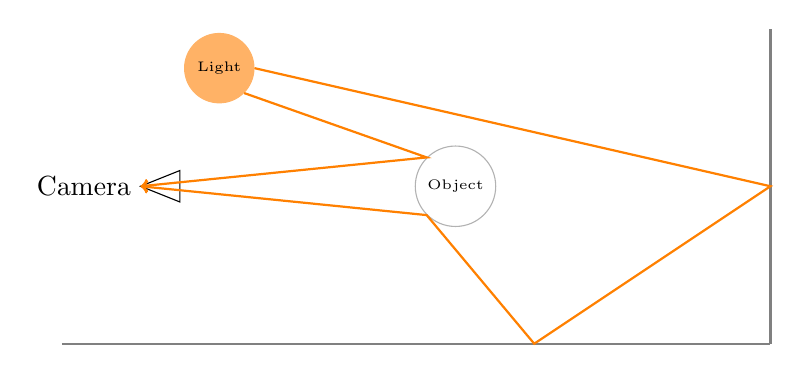
\begin{tikzpicture}
\draw[gray, thick] (-1,0) -- (8,0); %floor
\draw[gray, thick] (8,0) -- (8,4); % wall
\node[draw, circle, minimum size=1cm, draw=gray!60] at (4,2) (obj){\tiny Object};
\node[draw, circle, minimum size=5mm, draw=orange!60, fill=orange!60] at (1,3.5) (sun){\tiny Light};
\draw[black] (0,2) -- (0.5,2.2) -- (0.5,1.8) -- cycle node[anchor=east] {Camera}; % camera
\draw[->,orange,thick] (sun.south east) -- (obj.north west) -- (0,2); %direct ray
\draw[->,orange,thick] (sun.east) -- (8,2) -- (5,0) -- (obj.south west) -- (0,2); %indirect ray


\end{tikzpicture}
\label{raytracing}
\caption{The direct illumination is a combination of the light source properties and the object material. The indirect ray is a combination of the light source properties and the material of all the surfaces it collides with}
\end{figure}
\end{center}
\subsection{Indirect Illumination}
A product of the reflective nature of surfaces results in 'indirect lighting', an effect that is extremely difficult to capture in real-time rendering. The incoming light on a surface is made of photons arriving directly from light sources as well as photons being reflected from other surfaces, as demonstrated in \ref{raytracing}. Often when rendering is expensive it is appropriate to approximate the lighting in the scene to contain only 'direct' and 'environment' lighting. In this approximation, all objects are lit by the environment light, which represents an approximate light in all directions at all points in the scene. This is very cheap to render, as provided there is no direct lighting, all points on a surface recieve a constant amount of light. Direct lighting refers to lighting objects based on their proximimity to a given light source, ignoring shadows that would require calculating intersections between the light and the surface. Unfortunately this approximation results in very unconvincing images as in reality the light at a point is made up of all the photons being reflected from that point. The Phong shading model ignores the effect of photons being reflected many times within a scene, and so misses much of the subtle detail. A common way of calculating indirect lighting is 'Global Illumination', which involves tracing the paths of many light rays from light sources as they are reflected within the scene. To save computation it is often performed in reverse, where rays are drawn from the camera and reflected a constant number of times. The illumination of the final reflection is then computed from the direct lighting, which is then passed between the reflected surfaces to achieve the approximate lighting at the original scene point.
\subsection{Environment Maps}
Global illumination is a very expensive procedure and innapropriate for real-time rendering, where other approximations can be used. One such approximation is an 'Environment Map' or 'Environment Probe', first used for reflection mapping in computer graphics in 1976 \cite{Blinn:1976:TRC:360349.360353}. This can be thought of as a panorama image at a single point, capturing both the direct and indirect light, as shown in \ref{environment map}. In its simplest form, a designer would digitally draw a spherical image representing the environment to approximate the reflectiveness of objects. This technique was extended for use in the film industry, where environment maps were manually captured using composite photographs\cite{Debevec:1998:RSO:280814.280864}. While this cannot be used for every point in the scene, it is fair to assume that nearby objects have similar incident lighting. A common application is to use a large environment map to represent the lighting in outdoor scenes, where the main light source is the sky. This results in a vast improvement over a single Environment/Direct light combination, while still being inexpensive to compute. Furthermore, multiple environment maps can be blended together to roughly represent the lighting across larger scenes, often in combination with other approximations such as baked lighting.
\newline
A benefit of 'Environment Maps' is that rather than being computed, they can be captured from real-world data. This is a technique often used in films to apply the lighting from a set to virtual additions. This is achieved by taking photographs of a reflective sphere under different exposures to capture a range of lighting intensities. These images can then be composited to capture the range of light in a single format. By using a sphere, which has known geometry, it is easy to invert the image into a High Dynamic Range panorama. It is essential to use an HDR format, as RGB captures only a very narrow range of light intensity.
\begin{center}
\begin{figure}
\centering
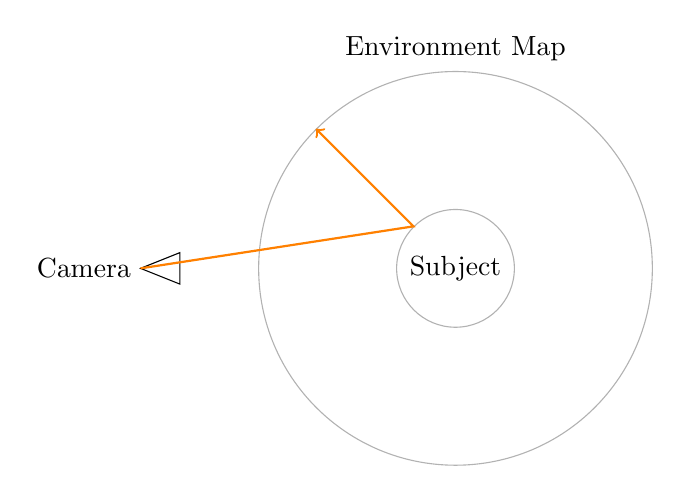
\begin{tikzpicture}
\node[draw, circle, minimum size=5cm, draw=gray!60] at (4,2) (env){};
\node[above] at (env.north) {Environment Map};
\node[draw, circle, minimum size=1cm, draw=gray!60] at (4,2) (obj){Subject};

\draw[black] (0,2) -- (0.5,2.2) -- (0.5,1.8) -- cycle node[anchor=east] {Camera}; % camera
\draw[->,orange,thick] (0,2) -- (obj.north west) -- (env.north west); %direct ray


\end{tikzpicture}
\label{environment map}
\caption{An environment map being used to render a sphere to the camera. This process is reversed with a perfectly reflective sphere to obtain the environment map}
\end{figure}
\end{center}
\section{Augmented Reality}
\subsection{AR in Film}

Augmented Reality is an extension of computer graphics and computer vision, where virtual objects are rendered on a real video stream to appear as if they are part of the original scene. This creates additional challenges as many of the parameters that are used in computer graphics are not available. While the material and geometry of the added objects is known, the geometry and lighting of the real scene must be estimated or manually recorded beforehand. The latter option tends to be used in films, where the layout of the scene and camera movements are known beforehand. In this case the geometry of the scene can be measured and recreated in 3D modelling or CAD software for a virtual approximation. Similarly, the lighting at points in the scene can be captured using a light probe, often a reflective sphere, and taking composite photographs at different exposures. This process results in an 'Environment Map' which captures the color and intensity of all the incoming light at a single point. With this data, additional characters can be rendered entirely in the virtual space, interacting with the approximated geometry and being lit by blended combinations of light probes across the scene. Provided that the virtual camera moves exactly as the real camera, the added object can be masked and overlaid onto the original video of the scene. To aid this process it is possible to estimate a cameras motion by tracking the movement of stationary markers within the camera view. Originally this would be achieved by placing deliberate high-contrast markers on the set, in places that would be covered by virtual characters or could be hidden easily.

\begin{figure}[H]
\centering
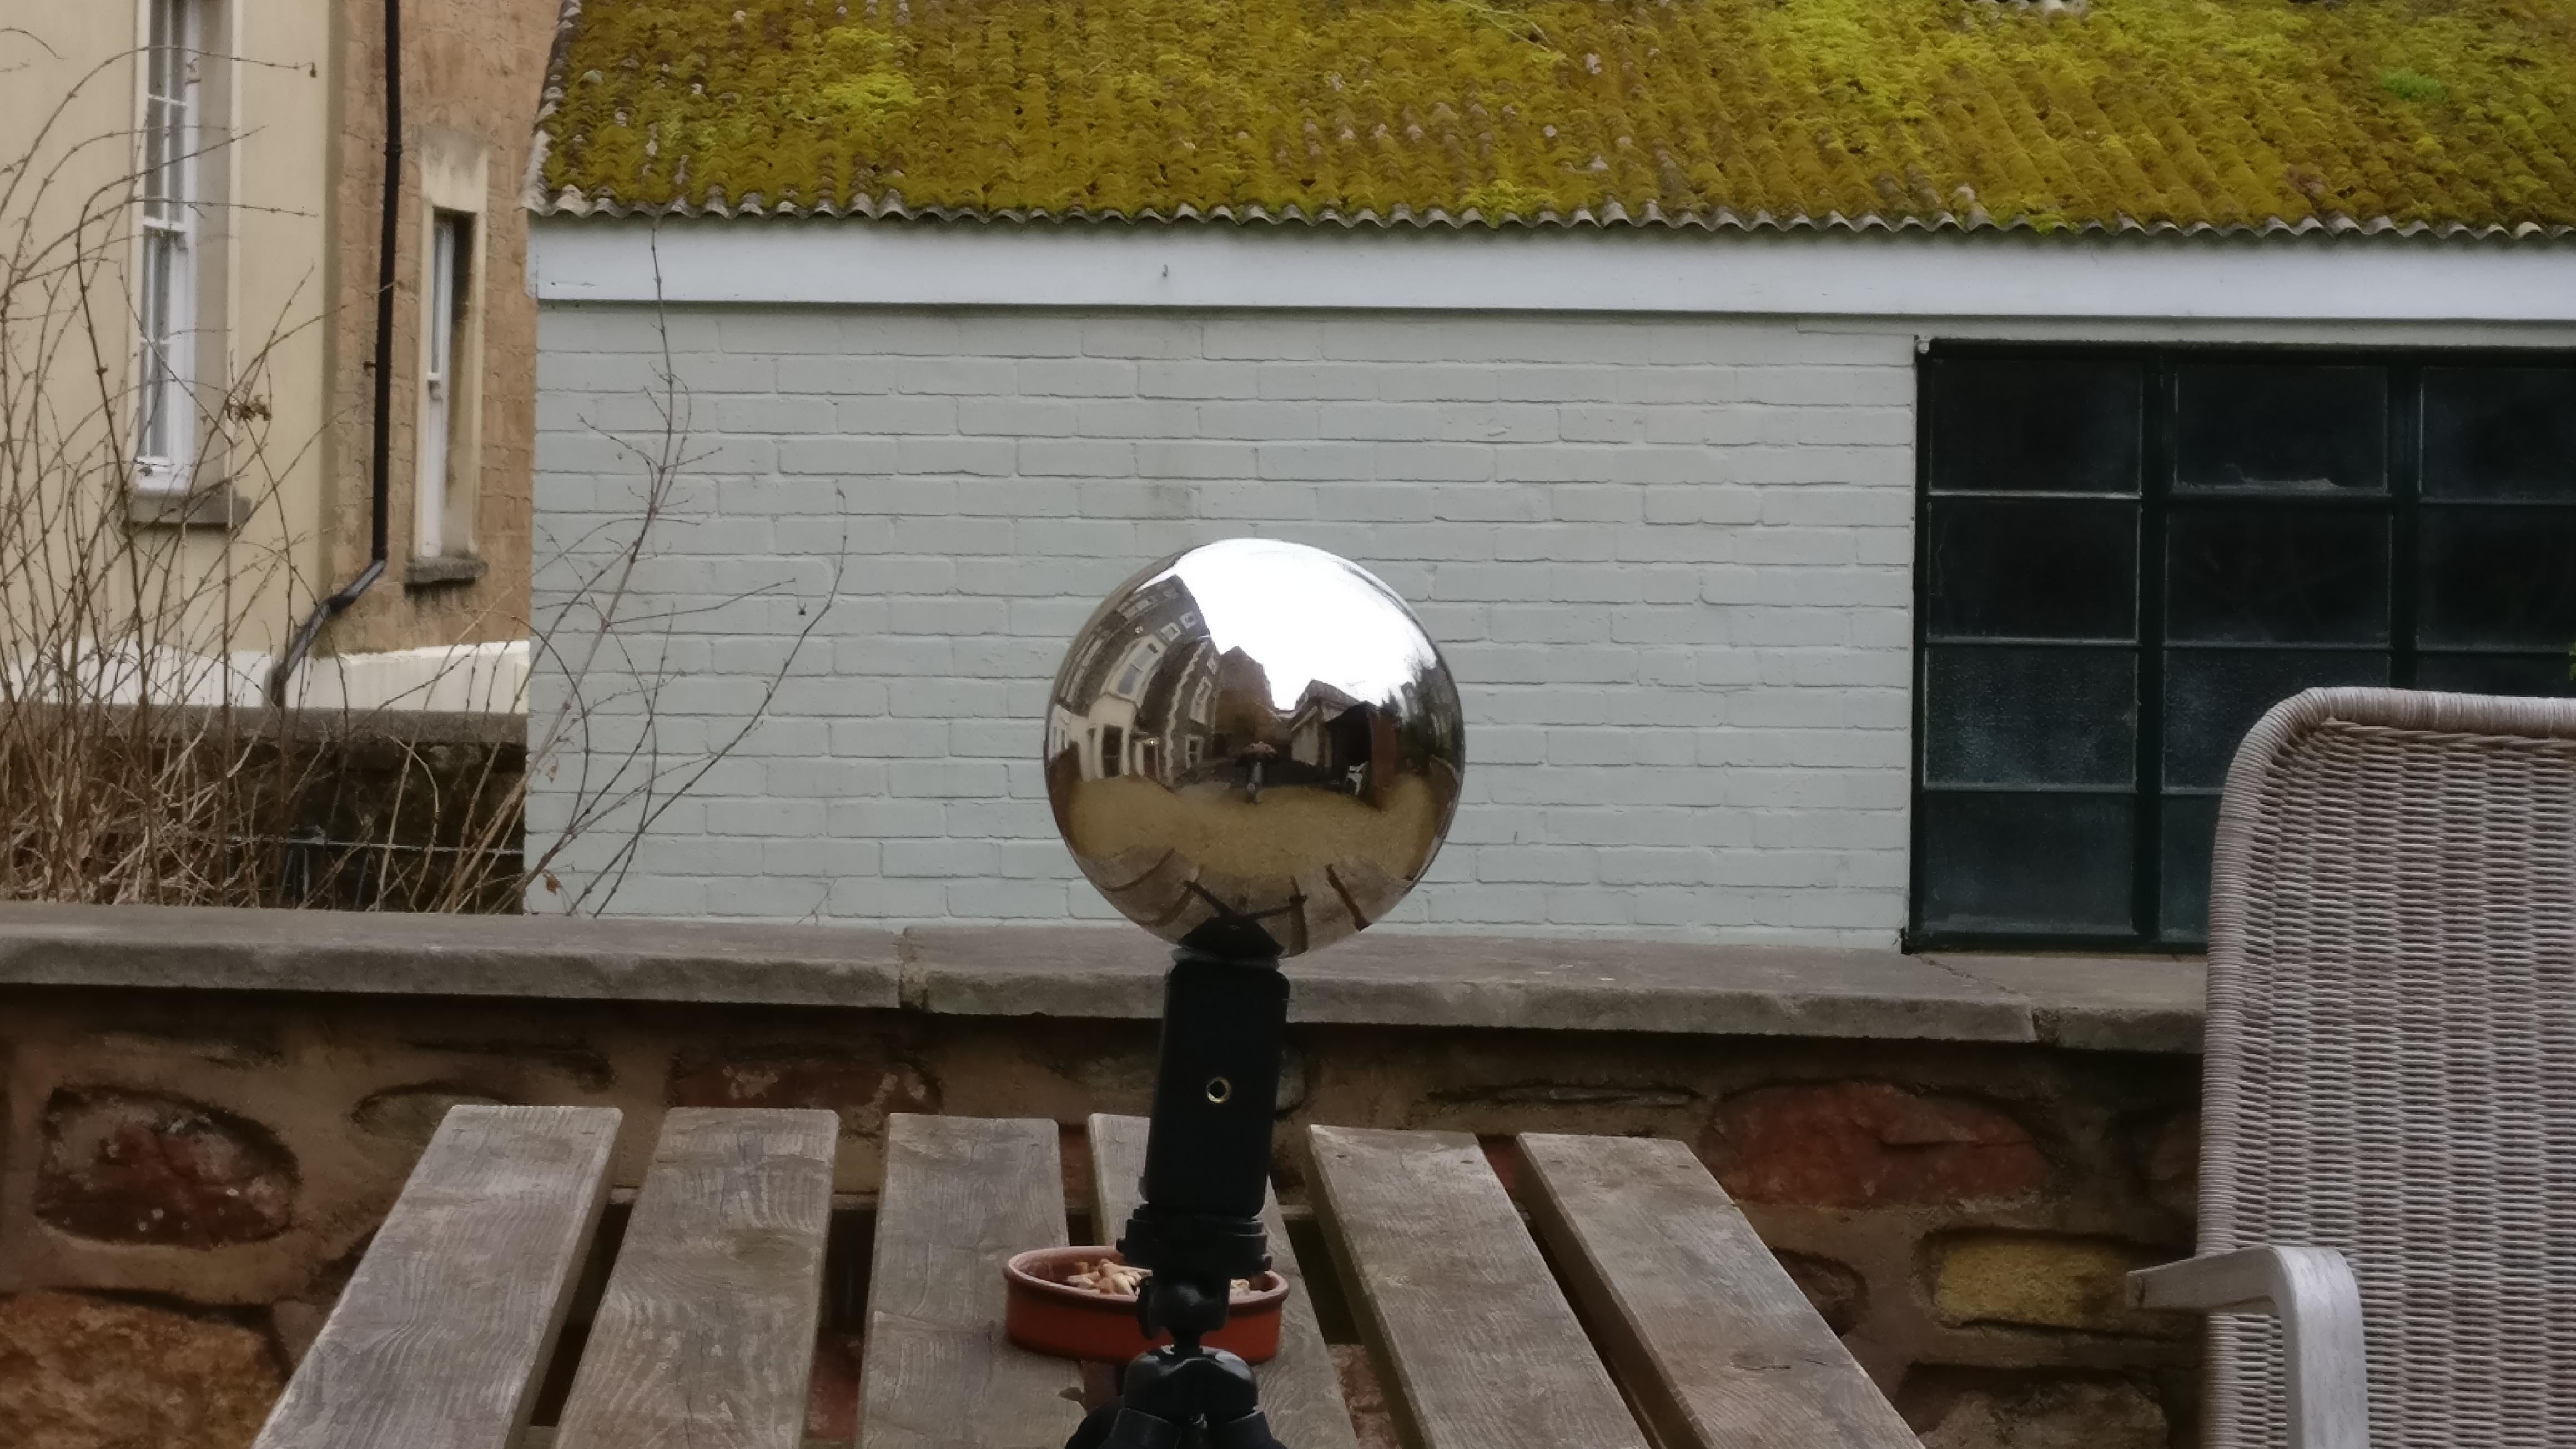
\includegraphics[width=7cm]{images/envmap}
\caption{A mirror sphere used to capture Environment Maps}
\end{figure}
\subsection{AR on mobile}
In live AR, as is becomming common in mobile applications, the scene data must be approximated entirely from data gathered from the devices sensors. Geometry estimation is performed using a process known as Salient Localization and Matching, which can be used to track the movement of a camera through a 3d environment while also mapping it. SLAM relies on finding similar points from multiple camera views, with the assumption that these points share the same position in 3D space. If static geometry is assumed, then the relative position of these tracked points can be used to build a 3d model or point cloud. Furthermore, groups of points that move together can be used to identify camera translations. SLAM is used extensively in the field of robotics, often using stereo cameras such that scene points can be calculated at every frame of an incoming video stream.

Tracking the camera tends to be the easier task, provided enough contrasting geometry and colors are part of the image to be used as salient points. All commercial AR solutions are able to achieve camera tracking to some degree, and so keep virtual objects in the same position in camera space. Building a 3d model of the scene is far harder however, with full point cloud representations unsuitable for low-power devices. The comprimise often used is identifying flat surfaces such as floors and walls to place virtual objects on.
\begin{wrapfigure}{r}{0.25\textwidth}
\includegraphics[width=4cm]{images/ar_example}
\caption{Example of Apple's ARKit lighting estimation in IKEA 'Place'.}
\end{wrapfigure}
\subsection{Lighting Estimation}
Another scene parameter that must be estimated is the lighting. Unlike geometry estimation which has significant uses in the field of robotics, solutions for lighting estimation tend to be more rudimentary. For real-time estimation, especially on mobile devices, it is common to simply pick the fastest approximation to maximise performance. In fact, mobile graphics hardware is far less powerful than what is used in the film industry, meaning that even perfect lighting representations may result in an unrealistic image. Nonetheless, mobile graphics hardware continues to improve and the quality bottleneck for AR will eventually shift to lighting estimation. In the case of shadows and reflective objects, good lighting estimation is a necessity. One fast approach is to simply take an intensity average across each incoming video frame, and use this to determine the overall brightness of the image. This is very approximate, and ignores light direction and colour but means that superimposed objects do not appear overly bright in dark areas and visa versa. There are also some techniques that make use of machine learning to estimate incoming light direction given some basic constraints light a single light source (usually outside), which restricts the possible incoming light or strictly portrait images, which reduce the possible scene geometry and materials.
\subsection{Human Scene Understanding}
The difficulty of these tasks arises from the fact that lighting, material and geometry are linked unknown parameters, and so an understanding of one is required to estimate the other. For example a red sphere may appear so because it is painted red, or because it is reflective and the lighting of the scene is red in tone. In fact this problem is the basis for many optical illusions, as it is sometimes difficult for humans to determine what exactly they are seeing under certain conditions. Humans share most of the properties of a moving mobile AR device, yet are able to infer properties of the environment under most circumstances. We achieve this by making assumptions and approximations while also utilising prior knowledge and a semantic understanding of the world around us. It is these features that we must formalise and exploit if we are to build convincing AR tools.
\newline
One feature that humans and computer vision sytems can exploit is shadows, where the light from a light source is blocked from reaching it's destination. In the case that we have an object of consistent shape and material such as a flat table, it is sensible to treat significantly darker patches on the surface as shadows. If we can find the object that is casting the shadow, it can be trivial to triangulate the light source. However, this technique is only accurate if there are no invariances in lighting across the scene that could result in changes in brightness across surfaces without explicit shadows. This model is still useful however, especially in outdoor scenes where we can treat the sun as a single light source, approximately equidistant from every point in the scene. In this case, any darkening on objects of the same material must be caused by shadowing. In indoor scenes we cannot make this assumption; often there are multiple light sources, which are close enough to the objects in the scene to cause differences in direct lighting. However in indoor scenes we have other consistencies to benefit from such as more uniform geometry. When we consider indoor scenarios, especially those likely to be applicable to AR and film we find that there are regular flat surfaces such as floors and furniture that are reasonably consistent in geometry. While the assumption that the light source is infinitely far away doesn't apply here, we are able to restrict light sources to likely directions, such as artificial light from bulbs above or natural light from windows. While these assumptions can aid in lighting prediction, it is still extremely difficult to build a robust lighting estimation system for indoor scenes, resulting in the simplified techniques used in todays AR platforms.
\newline
Often the reason humans find it easy to understand the light in a scene is because of a semantic understanding. While we do not know the geometry of every room we enter, we are able to recognise consistencies that we have encountered before. While a single image patch could technically be any combination of material, light and geometry we can restrict the likely combinations by recollecting previous times we have seen something similar. We understand, for example that surfaces with dramatic variances in color and light intensity are more likely to be a reflective metal than to have those diffuse colour properties. Similarly if we see an orange tinted outdoor scene we know to assume that it is probably due to the color of the sky, because we recognise that known surfaces like grass or concrete are not naturally that colour.
\section{Depth Imagery}
\begin{figure}[H]
\centering
\includegraphics[width=8cm]{images/Stereo_Matching}
\caption{Example of Stereo Imagery. Points that appear further apart in the 2 camera places are further away from the camera due to parallax.}
\end{figure}
\subsection{Depth Cameras}
One of the most important components for scene understanding tasks is that of geometry. In the field of robotics especially, it is vital to be able to understand the placement of obstacles within the scene, while being tolerant of material and lighting changes. This problem is often paired with the task of motion or camera tracking, such that an actor can understand how they fit in 3d space. Furthermore, many of the techniques for lighting estimation previous mentioned require some understanding of the geometry of the scene. Geometry estimates tend to come in the form of depth and surface normals, which represent the distance from the camera and the surface normal direction (usually n camera space) for every pixel on the screen.
\newline
One method for collecting depth information is to use a depth camera, with specialized hardware to calculate depth for every pixel. An example of this would be the Microsoft Kinect camera, popular in computer vision tasks for it's low cost. This calculates depth by projecting a pattern of infrared points onto the subject, and measuring how the distance between the points changes as objects move within the scene. For many cases this is inpractical, as the depth resolution is limited, and it's reliance on IR makes it unusable outside. It is however an excellent tool for collecting ground truth depth data for other systems \cite{Khoshelham_accuracyand}.
\newline
Another approach for capturing depth information is the use of stereo cameras, which record two seperate images of the scene. If the relationship between the two cameras is known, and the views of the cameras intersect, the epipolar constraint can be used to calculate the distance of every point from the camera. In this case, the center point of each camera view projects onto a unique point in the other's view. If corresponding image points can be found, the epipolar constraint can be used to find the exact projected 3D point. Even if the camera properties are unknown, if matching image points can be found, the relative depth of the images can be calculated.

\subsection{Stereo Matching}
Finding matching points between two images is a difficult problem, as some points may be duplicated or even occluded. This requires some form of stereo matching, often involving the comparison of image patches. One technique is to find the Normalized Cross Correlation of image patches, but this technique is very slow, and the accuracy of the results depends on the size of the image patch. Similar block-matching methods like Sum of Squared Differences or Sum of Absolute Differences can be used but suffer the same accuracy penalty. There is a tradeoff in most stero matching algorithms between reliability and accuraccy, as detecting the movement of single pixels is difficult, as on flat surfaces the value may not change for large regions. Similarly small image patches are affected by changes in lighting and material. On the other hand large sizes can only calculate a lower-resolution depth image. \todo{Graphcut} More modern techniques such as \cite{7780983} use CNNs to extract features at different granularities, before attempting to find the disparity between them. This has shown to be incredibly effective, combining the effects of global methods and block matching. If the network is carefully, the matching can take advantage of feature similarities like uniform geometry.
\section{Machine Learning}
Because the complicated nature of semantics it is very difficult to create a system that explicitly relies on finding known patterns between scenes to cover all cases. For example it would be viable to create a system tht extracts IKEA furniture from scenes, and uses the known geometry and material to treat the furniture as sparse light probes. This would not be able to account for scenes without known furniture, outdoor scenes or even scenes where the furniture is partially obscured. Instead it is a sensible approach to consider machine learning. Machine Learning is a field of Computer Science that involves training the parameters of a system on data to make predictions. By taking known input and output pairs it is possible to adjust the parameters of the system such that it can generalise to inputs with unknown outputs. In our case it would be possible to train a model to take input images, either raw or preprocessed, and output some representation of the lighting. Traditional ML models such as the Support Vector Machine are able to learn a given number of parameters from some input features. These features could be extracted from the image, such as the average intensity or the dominant frequency in the fourier domain. These models are easy to train and can produce very predictable results, but require the designer to explicitly provide a set of features that they believe can be used to seprerate or define the different outputs. For example if our task was to predict whether a given image was 'indoors' or 'outdoors' we have restricted our problem to binary classification - our outputs are known. It would then be feasible to provide some features, such as average colour or number of colour clusters above a threshold to then train an SVM.
\newline
\subsection{Deep Learning}
If we wish to predict a more complicated lighting model we must be able to take into account many more features than what we can feasibly define by hand. In this case we can look to the field of AI, and explicitly Convolutional Neural Networks. In the field of AI it is possible to train a model without explicit features, by using an approximation of neural dynamics in real brains. In broad terms, we programmatically create a series of connected neurons in a layered structure, with each neuron having a number of inputs and some number of outputs. The neurons have a very simple behaviour - they multiply each input by some 'weight' and provide the accumulated result as the output.
\[y_k = \sum_{j=0}^{m}{w_{kj}x_j}\]
By training on known results we can adjust these weights so that the final neuron layer (which matches our desired output data shape) contains the desired output.
\newline
Convolutional Neural Networks are a recent development in AI that allows for reasonably fast AI models that take images as input. Rather than having a neuron for each colour of each pixel, we can instead learn the weightings for a 'convolution'. A convolution, in this context, is a function which can be passed across an image to extract features,
\[\sum_{n_1=-s}^{s}{\sum_{n_2=-s}^{s}{f[n_1, n_2]\cdot g[x-n_1,y-n_2]}} \]
and often resembles a SxS matrix. Convolutions are used frequently in computer vision, as they are an efficient way of computing many popular image features such as Harris Corners or Sobel Edges. In a CNN we intend to learn the weights of many convolutional matrices to quickly extract featured from the input image. Furthermore we are able to pass further convolutions across the results from previous convolutional layers to learn more complex features. For example the first layer could extract edges while a second layer extracts the presence of 'X' shapes. CNNs make it possible to train deep and complex models on image data, resulting in robust models that often vastly outperform their traditional ML counterparts.
\newline
The performance of CNNs is heavily impacted by the choice of metrics used to decide the weights and behaviour for each neuron. When given inputs and weights a neuron may or not fire depending on an 'activation function'. In biological neurons, this is a complex nonlinearity that is difficult to efficiently capture in artificial neural networks. Instead we use approximations like 'Relu',
\[f(x) = max(0,x)\]
to decide whether to fire after calculating the output value. Furthermore during training it is important to consider how to adjust the weights to converge on the optimum. For this we use a 'Loss Function', which computes an error value given the desired, or ground truth, value and our models prediction. The rate of change of this erroris then used to iteratively adjust the weights of each neron based on its influence.
\subsection{Image Regression in Deep Learning}
The prime application of CNNs has been in image classification, where the model must distinguish between a set number of classes. However it is possible to use CNNs for regression tasks that output other images using the concept of 'deconvolutional' layers. These learn an interpolation matrix that increases the dimensionality of the input. Popular image regression architectures often involve a series of convolutional layers followed by a series of deconvolutional layers. The aim of the convolutional layers is to learn a deep representation of the content of the image, often removing the original spatial dimension. Rather than 'shallow' features like edges or colours, these features ideally represent some 'understanding' of the scene such as presence of some object or shape of the environment. The deconvolutional layers can then interpolate this data into a new image that will often share many common features with the original. For example in style transfer, the convolutional layers attempt to extract the content of the image while the deconvolutional layers interpolate the image features with weights representing some artistic style.

\subsection{Training Data}
The difficulty in the application of CNNs often lies in the 'training' stage; while a deep enough network should be able to learn a mapping for any function, the difficulty in providing data to capture every case increases with the problem complexity. If a network is trained to recognize images of dogs, it will only be able to learn features from dogs that it has seen as input. As a result, if a new dog is provided that lacks some of the features of the training data, it may be missclassified. Regression tasks in particular attempt to learn a complex funtion and so need a vast amount of training data to be able to generalise. This becomes problematic where the training data is hard to collect and classify.
\begin{wrapfigure}{r}{0.4\textwidth}
\includegraphics[width=5cm]{images/example_synthetic}
\centering
\caption{An example of syntethic data used for our work.}
\end{wrapfigure}
In the case of image classification, many photographs can be taken and marked with their intended class. With image regression this can become an extremely laborious task as the desired output needs to be extracted by hand. Often there are large datasets already available that can help speed up the process, especially if the datasets are labelled, or if features can be extracted by hand. However it is simply necessary to manually create a dataset to train a network to face a new task. Fortunately there are still some steps that can be taken to accelerate this process, such as data augmentation. This usually involves manipulating some training inputs in such a way as to introduce variances while maintaining the classification, and can greatly increase the amount of data available.
Another approach is to create synthetic virtual data, by rendering new images. It is important to note however that the synthetic data must be accurate enough such that a model trained on it can generalise to real world data. It is often sensible to mix real world and synthetic data when training a model for the best results.



% -----------------------------------------------------------------------------

\chapter{Technical Background}
\label{chap:technical}
\section{Commercial Lighting Solutions}
\subsection{Film\&TV}
Lighting solutions in the film\&TV industry tend to involve precalculating or precapturing the lighting in a scene before adding virtual characters. In the film 'Flight of the Navigator', Randal Kleiser first demonstrated the technique of reflectance/environment mapping in a feature film \cite{navigator}. Here the reflectance was computed using a simple rectangular photograph, although more accurate implementations used spherical photographs of a gazing ball. Later films used a semi-automated system for capturing HDR environment maps using a rotating fisheye-lens camera. Once placed, the camera was able to take shots at multiple angles and at a range of exposures, before compositing the shots together to produce a usable HDR lighting map. Often these HDR maps are not used in isolation, but along with footage of a proxy for the virtual addition, so the filmmakers can qualitatively measure how the materials react with the set lighting. These techniques allow filmmakers to capture an approximation of lighting with limited camera equipment and makes it easier to create complex panning and dolly shots of scenes with real and virtual elements, which would otherwise require a green-screen. Over time, camera equipment has become more advanced and it is faster to take high quality shots at multiple exposures. As a result, later films such as 'The Curious Case of Benjamin Button' are able to utilise multiple lighting probes to illuminate characters. By taking lighting samples across the scene, virtual characters can then be lit partly according to their position in the world by blending environment maps together. This creates a more convincing final render as the approximate indirect lighting from nearby objects becomes more apparent. The downside of these hollywood techniques is that the lighting data must be captured beforehand for every environment used. This is a long, laborious and expensive process as the cameras required to take accurate shots at different exposures need to be extremely accurate to produce correct composites. It is also important to note that compositing images is difficult and also requires human input to match black levels, tones and camera properties that are hard to automate.
\subsection{Mobile AR}
Recent commercial AR platforms do contain some level of lighting estimation from input video data. Apple's ARKit is able to estimate the colour and intensity of the ambient lighting in some scenes \cite{arkit1}, by analyzing the pixels of the incoming video frame. This technique adds some realism to AR applications, as objects can be dimmed or brightened with the scene, so as not to stand out. However this is a very rough estimate of lighting, and contains no directional information or approximation of indirect illumination  Google's ARCore has similar functionality, taking an average of the luminance values across the video to estimate the intensity \cite{Debevec:1998:RSO:280814.280864}. It is possible to estimate the light direction from a face tracking scene however, by using the tracked face as a light probe. By using a face, the application is able to restrict the possible lighting scenearios to a range of likely geometries and materials that make up human faces. The platform is able to produce not only the primary light direction and intensity, but also an approximation of the environment lighting as spherical harmonics. While incredibly useful for some application such as the retouching of portrail photographs, the technique is not robust to different scenes as it relies on the approximation of some known geometry.
\begin{wrapfigure}{r}{0.4\textwidth}
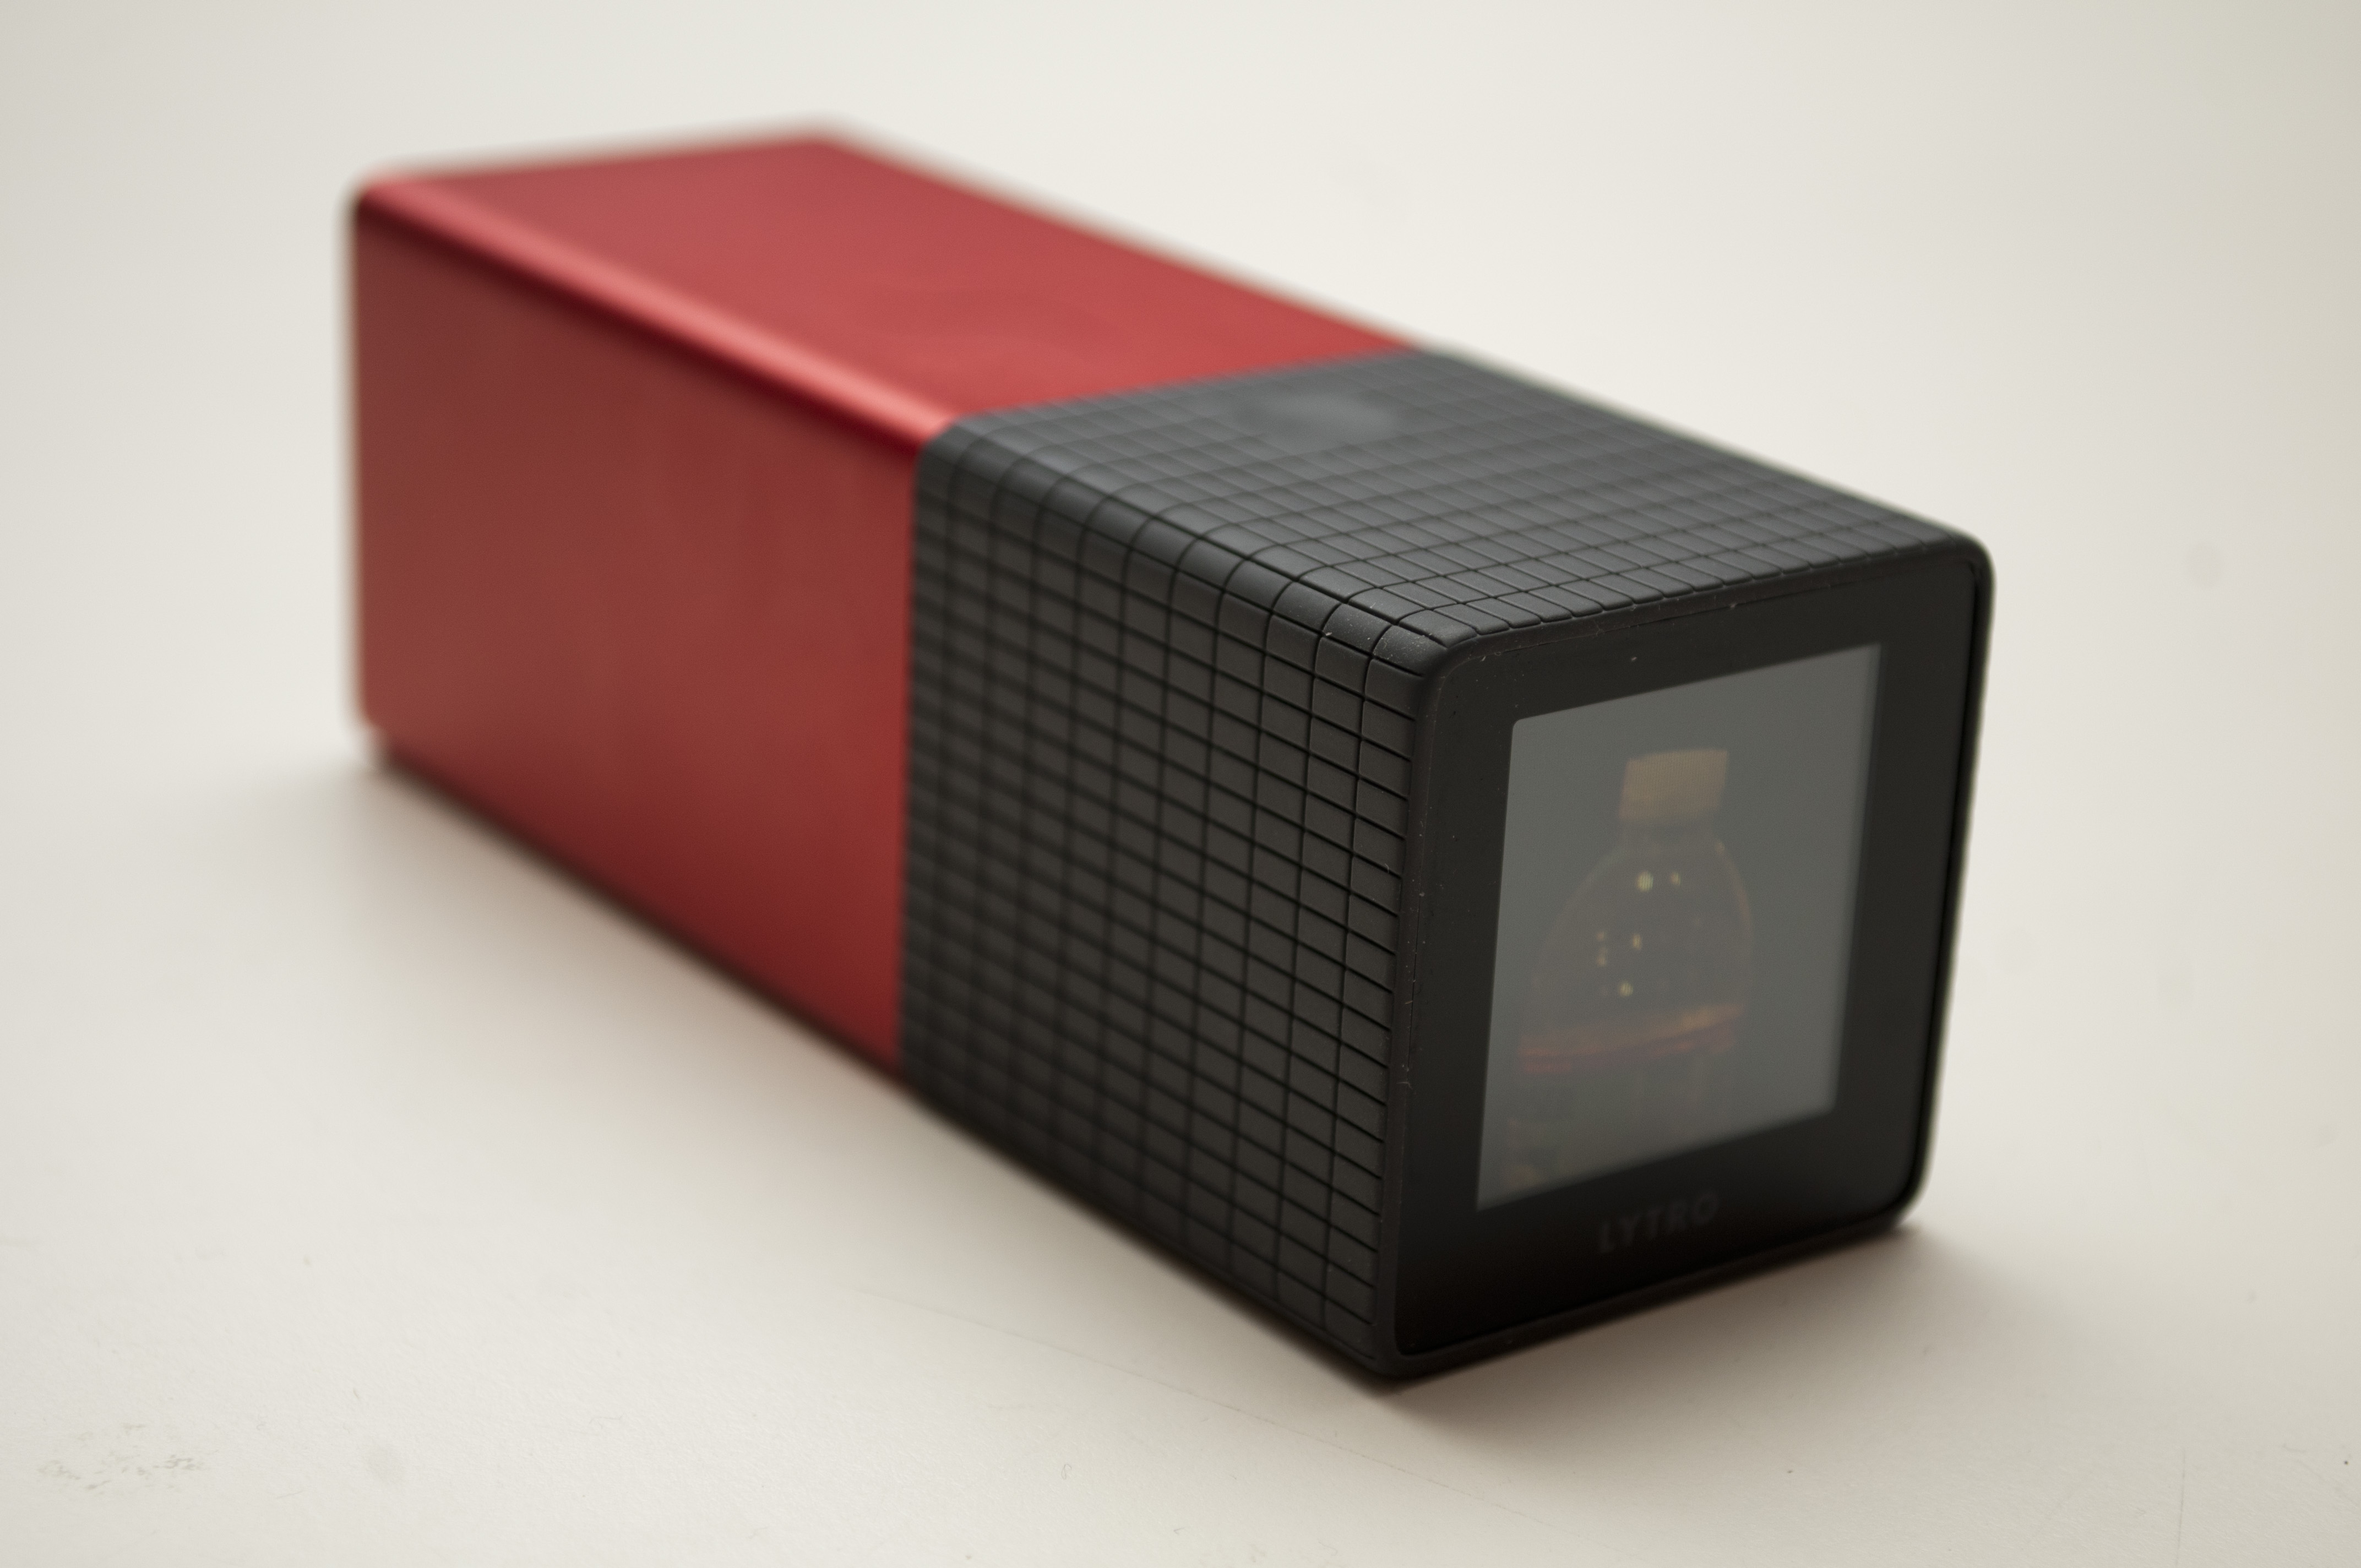
\includegraphics[width=5cm]{images/lytro}
\centering
\caption{A commercial light-field camera from \textit{Lytro}}
\end{wrapfigure}
\newline
Upcoming AR applications are experimenting with new methods of integrating the scene lighting with virtual augmentations. Magic Leap is making use of tailored hardware called a 'Light Field' camera, which involves the use of an array of microlenses to capture additional information from the scene. Each microlens is able to capture information from multiple camera points, so that extra depth and lighting information can be extracted from the frame. This is a significant improvement on IR depth cameras such as the Microsoft Kinect, which can't be used outside. By extracting depth, and therefore surface geometry information, it is far easier to reason about the reflectance of objects within the scene and estimate the lighting. However, light-field cameras are extremely expensive and inpractical for mobile AR. Most mobile devices contain normal high quality cameras as well as accurate intertia sensors, which can be used in combination with stereo matching for a similar depth estimation model.
\section{Lighting Estimation Research}
\subsection{Direct Lighting}
Early techniques for lighting estimation were able to find the direction of a single primary light source, under significant constraints. In \cite{990650}, Peter Nillius and Jan-Olof Eklundh were able to estimate a single light direction, provided the input image contained an appropriate lambertian surface.
\begin{wrapfigure}{l}{0.5\textwidth}
\includegraphics[width=5cm]{images/Contour}
\centering
\caption{A self occluding contour. The surface normal is orthogonal to the camera ray, and so the brightness of resulting pixel compared to the rest of the surface gives a good indication as to the illumination arriving from that direction.}
\end{wrapfigure}
By making use of an 'occluding contour' it is possible to infer some detail of the geometry, as the surface of the visible edge of a contour that occludes itself will always be perpendicular to the view direction of the observer. Using the lambertian lighting model, along with the edge intensity it is possible to make a prediction using a bayesian network for the incoming light direction. This is a simple method that exploits inherent properties of real geometry, but has too many prerequisites to be practical. While it captures direction, it also ignores colour, intensity and any indirect lighting. Similarly, Varma demonstrates a technique to estimate the lighting direction from textured images \cite{1315030}. If the surface is constrained to be a gaussian surface with uniform albedo, the incident light direction can be estimated by the shadows cast by the height changes in the material. While also very constrained, it is shown that even strict models can generalise to produce useful results in this field.
\newline
There has been some work in inverse lighting specifically for the rendering of AR objects, notably that of \cite{Aittala2010}. In this work the user must simply provide a ping-pong ball, representative of a lambertian sphere, while the least-squares algorithm is performed on the lighting equation, using features of the sphere as constraints. This results in an approximation of illumination as a series of point lights and spherical harmonoics which can practically be used for rendering. The downside however is that the process of presenting the system with a known ball can take upwards of 20 seconds, and the resultant lighting is suitable for only primarily diffuse objects. This does however demonstrate how powerful even basic knownledge of the geometry and material of the scene can be for deriving the lighting.
\subsection{Outdoor Lighting}
In \cite{Lalonde-2009-10350}, Lalonde et al. are able to estimate a more complete set of parameters for environmental lighting from single outdoor photographs. By segmenting the image into sky, ground and vertical surfaces, and extracting features like shadows, the authors are able to reliable predict the sun's position. While very robust for outdoor applications, this approach does not consider light intensity or colour. Furthermore, the reliance on outdoor scenes restricts its usage in AR.
Scott Wehrwein et al. demonstrate a technique for sun direction and shadow detection from multiple input images \cite{7335515}. They use illumination rations to extract shadows, after constructing a sparse 3D representation of the scene from stereo matching of multiple images. By exploiting shadow boundaries on the derived surface normals, it is then possible to determine the light direction. This work shows how multiple views can be used to infer knowledge of the geometry of the scene, to make the problem of lighting estimation more constrained. However, like previous work it assumes a perfectly lambertian surface and clear outside conditions, restricting the possible lighting conditions significantly.
\subsection{Shadows}
It is clear that estimating a full representation of the illumination within a scene is very difficult given the number of unknowns. However predicting only the direct light sources is still very valuable, as this makes up the majority of the light within a scene, and can be combined with image colour values to give an approximation of the indirect lighting. Shadows are a good indicator of the direction and intensity of direct lighting. They not only give some indication of direction based on shape, but also the intensity through the contrast of colour values between areas that are shaded and unshaded. Takahiro et al. demonstrate techniques for recovering illumination from shadows in \cite{1315013}. This work compares two methods, \textit{Spherical Harmonics} and \textit{Haar Wavelets} for estimating the illumination from cast shadows on known geometry. Spherical Harmonics are function defined over a whole sphere, and are useful for defining the light reflectance at a point, as in Global Illumination. The work demonstrates how this method fails to capture higher frequency illumination values, and presents \textit{Haar Wavelets} as an alternative. This method is able to approximate functions as a series of linear combinations of Haar functions, and is able to more efficiently capture a higher range of light frequencies at a point.
\subsection{Experimental Methods}
An interesting approach from Microsoft Research \cite{xia} attempts to reconstruct the shape and reflectance of an object from a video with known motion and camera pose. This is achieved by decoupling the estimation of geometry from the estimation of illumination, and refining initial estimates over a series of video frames. While the lighting is not known in the scene, the camera pose and motion must be known and so this work is only applicable under carefully controlled environents. However it effectively demonstrates how multiple views of an object can be used to refine predictions of scene understanding, under the reasonable assumptions of static lighting, material and per-object geometry.
\newline
An emerging trend in lighting estimation research is the use of 'light fields' as a way of representing the light on an entire scene. A light field represents the radiance of light flowing in each direction in each point in space, resulting in a 5D function. Capturing and storing light field data is difficult as for a given area, light must be sampled in all directions at all points, which is impractical using traditional cameras. The use of microlens light-field cameras, which sample incoming light rays at a range of angles, has made capturing light-fields much less costly, resulting in datasets becoming available such as that of \cite{hazirbas17ddff}. Light fields require immense quantities of storage capacity and contain far more light information than is required in the field of AR, making their use inpractical. Instead most work has been centered around the estimation of light at a single point, either at the camera view or in the scene, that can be seen as a sparse sampling from the light-field.
\begin{figure}[H]
\includegraphics[width=3cm]{images/antinous_rgb}
\includegraphics[width=3cm]{images/antinous_lf}
\centering
\caption{An example of the extra data captured by light-field imaging.}
\end{figure}
\section{Deep Learning for scene understanding}
\subsection{Geometry Estimation}
To calculate the lighting of a scene, some assumptions or approximations must be made about the material or geometry to constrain the problem. It is therefore important to consider previous techniques to extract these features from images, especially geometry estimation which has significant applications in the field of robotics. In 2015, David Eigen et al. demonstrated a CNN approach to estimate depth, surface normals and semantic labels from single input images \cite{7410661}. Here they use a 'multi-scale' architecture, where outputs from early features passed as input to later deconvolutional layers, as well as subsequent convolutional layers. Multi-scale features can often lead to faster inference as important features are 'short-circuited' closer to the output, reducing the need for large deep layers at inference time \todo{Citation needed ;) }. The results of this work are extremely promising, and suggest that a single RGB image may be enough to infer a complex understanding of the scene. If it is possible to understand variations in the illumination and material in a scene to find geometry then it follows that it is possible to understand geometry and material to find illumination.  However the network shown is very deep and trained primarily on indoor scenes. Its use in the field of AR is limited, as the hardware is much more limited in terms of GPU resources. Furthermore while the network is able to predict depth and surface normals on a large scale, successfully finding walls and floors, it struggles with more complex geometry. Some progress has recently been made to improve performance in geometry estimation by incorporating more traditional SLAM techniques. In their work, Luo et al. show increased performance in stereo matching by including a dot product step \cite{7780983}. In stereo matching tasks, two images are used to compute a disparity map, which corresponds to a relative measure of depth due to the parallax effect. This work uses a siamese network, where the same features are extracted from each of the two images. As a result, using a dot product computes a similarity between the two sets of feature outputs. This is equivalent to the \textit{Cosine Similarity} of the image vectors, provided they are normalized. This greatly reduces the number of layers that would otherwise be required to map the input image to output disparity map, while still producing accurate results.
\subsection{Synthetic Datasets}
With it's usefullness in robotics, geometry estimation has been a primary focus of scene understanding tasks. Geometry datasets are easier to source, with depth cameras becoming cheap and easily available. Other important information like material, texture, semantic class, albedo an many others are almost impossible to capture efficiently from real scenes using hardware. Instead these parameters must be hand labelled, which is expensive, slow and leads to noisy results. The recent availability of high quality synthetic datasets such as SUN-RGBD \cite{song2015sun} and the very recent Scenenet-RGBD \cite{McCormac:etal:arXiv2016} however, have provided more opportunities for learning scene parameters that are more difficult to retrieve from real scenes. For example, Rajpura et al. demonstrate how semantic segmentation networks can be improved by augmenting real data with the readily available synthetic data \cite{DBLP:journals/corr/abs-1709-00849}. Some networks must be trained entirely on synthetic data, such as that of Narihira et al. which utilises the syntetic MPI Sintel dataset to predict shading and albedo, which can't be captured by hand. Unfortunately, many synthetic datasets do not generalise well to real data, and it remains to be seen whether virtual scenes with the level of detail needed for lighting estimation can be rendered fast enough to be practical for research, although recent datasets appear promising.
\begin{figure}[H]
\centering
\includegraphics[width=16cm]{images/scenenet}
\caption{Example synthetic Scenenet RGB-D data, containing RGB, depth, semantic instance, semantic class and optical flow.}
\end{figure}
\section{Deep Learning for Illumination Estimation}
Most of the previous work has had to rely on significant assumptions for the scene to constrain the lighting to fit known phenomena, that can be exploited to estimate the illumination. It is clear that due to the unconstrained nature of the problem, that some assumptions about geometry, material and lighting must be made. Rather than making the required assumptions to fit a model, another approach is building a model to find and exploit assumptions from real data using machine learning. Given enough scene features and data it is possible to learn approximations and assumptions to produce a more robust model. In \cite{holdgeoffroy-cvpr-17}, Yannick Hold-Geoffroy et al. use a CNN-based technique to estimate sky parameters from outdoor photographs to a high enough degree of accuracy that virtual objects can be re-rendered. In this work, the output illumination model is constrained to the Hosek-Wilkie model with parameters representing the sun position, ground albedo and light wavelength. A dataset is then constructed by selecting small LDR sections of real HDR scene panoramas, resulting in a large number of sample photographs, and HDR lighting ground-truths. This work demonstrates extraordinary performance, but is limited in output format by the lighting model which is constrained to outdoor images with clear skies. This ignores the indirect lighting from scene objects and indoor scenes, but demonstrates how CNNs with the right data can be used to exploit more subtle image features to predict lighting.
\newline
There have been advancements in the field towards estimating the lighting in indoor scenes, such as that by \cite{Gardner:2017:LPI:3130800.3130891}. In this work, Gardner et al. use a very large dataset of indoor HDRI environment maps to train a CNN to predict the environment map at the cameras position. This environment map can then be warped to provide an approximate environment map for a given position. The resulting network is very accurate for predicting light direction and intensity, but fails to predict colours which must be provided for a user. Furthermore the network is very deep, making it difficult to deploy on mobile devices. While the warping operator user is innovative, it fails to accurately capture the lighting at points in 3d space, and instead provides a rough approximation. Finally, the produced lighting requires a manual tuning step if it is to match the scene in hue, though this is the still very promising work in the field of lighting prediction.
\section{Predicting Light Probes}
CNNs can exploit different features in a scene to determine lighting such as shadows or object reflectance. One example that uses the latter is 'Deep Reflectance Maps' \cite{RematasCVPR2016} by Konstantinos Rematas et al. In this work it is demonstrated that better accuracy can be achieved by constraining the CNN input to a specific feature, in this case a sparse reflectance map, provided the geometry is known. A reflectance map is mapping from surface normal direction to light reflectance in that direction. By taking the brightest pixel for every surface normal on an object, a sparse representation of it's reflectance can be built and fed to a CNN for interpolation. This work makes use of a large synthetic dataset but still results in good performance on real world data, allowing the researchers to then modify the shape of specular virtual objects while still maintaing a realistic surface appearance. An important feature of this work is that the researchers present results from reflectance maps produced from perfect surface normals, and from those produced by noisy estimated normals. It is demonstrated that the estimated normals are unsuitable for accurate reflectance mapping, and actually result in poorer predictions than a direct appearance-to-lighting network.
\begin{figure}[H]
\includegraphics[width=8cm]{images/reflectance}
\centering
\caption{The \textit{Deep Reflectance Maps} pipeline. Estimating the full reflectance map from the geometry and depth data allows for modification of the material.}
\end{figure}
This work was then extended for illumination estimation in 'What is Around the Camera', by using a precalculated sparse reflectance map in combination with a segmented background image. In this work, a full HDR environment map is predicted to a degree of accuracy that allows the superimposition of rendered geometry with fairly accurate lighting. Both of these works use a Convolutional-Deconvolutional approach to produce a new image as output. The limitations of this work however are due to required prior calculations rather than restrictive assumptions about the scene. While the network can handle objects of multiple materials, they must be segmented and seperate sparse RMs calculated. Furthermore the calculation of the sparse RM relies upon knowledge of the surface normals of the object being used. The researchers point to previous work \todo{Talk about this} on the usage of CNNs for surface normal and depth estimation but fail to demonstrate the accuracy of their work with these more noisy estimated surface normals. It is also apparent that there is significant data loss in the calculation of the sparse reflectance map, which makes significant assumptions about the object in question, ignoring the effects of shadows and how lighting changes based on both position and surface orientation.
\newline
These works demonstrate that if surface geometry is known, a network can be trained to accurately reproduce lighting conditions, using an object as a probe. However they point to 2 significant shortcomings that we attempt to address in this work. Firstly the use of sparse reflectance maps in isolation ignores a significant amount of useful information on the object that could be used to estimate the lighting. As a result, a direct approach of predicting illumination from a single image view can often outperform cases where the reflectance map is too sparse or the material is very diffuse. Secondly, modern surface normal estimation techniques from single images are not accurate enough to constrain the problem of lighting estimation. We believe that the use of a network that exploits multiple views of an object, provided the scene parameters remain constant, will be able to more accurately predict the geometry through learned stereo matching. Furthermore, a network that simultaneously learns geometry and lighting will be able to exploit more scene features such as shadows, that would otherwise be unavailable in an explicit reflectance mapping.
\newline
\footcite{https://www.disneyresearch.com/publication/face2light/}
\begin{figure}
\def\checkmark{\tikz\fill[scale=0.4](0,.35) -- (.25,0) -- (1,.7) -- (.25,.15) -- cycle;} 
\begin{tabular}{|c|c|c|c|c|}
\hline
Model & Geometry Prerequisite & Material Prerequisite & Direct Lighting & Indirect Lighting \\
\hline
Mirror Ball & sphere & mirrored & \checkmark & \checkmark \\
Nillius et al. & occluding contour & Lambertian & \checkmark & X \\
Varma et al. & Isotropic Gaussian Surface & Constant Albedo & \checkmark & X \\
Lalonde et al. & Outside with floor\& sky & X & \checkmark & X \\
Wehrwein et al. & Outside \& clear & Lambertian & X & X \\
\hline
\end{tabular}
\caption{Summary of current methods}
\end{figure}

% -----------------------------------------------------------------------------

\chapter{Implementing Prior Art}
\label{chap:execution}

\begin{wrapfigure}{r}{0.6\textwidth}
\centering
\begin{tikzpicture}
\node[rectangle, minimum size=4cm, anchor=north, draw=black!60](encode) {};
\node[below] at (encode.north) {Encode Block};
\node[rectangle, minimum size=2.5cm, draw=black!60, below=5mm of encode.north](loop) {};
\node[rectangle, draw=black!60, below=3mm of loop.north](conv) {Convolution};
\node[rectangle, draw=black!60, below=3mm of conv.south](bn) {Batch Norm};
\node[rectangle, draw=black!60, below=3mm of bn.south](relu) {Relu};
\node[rectangle, draw=black!60, below=2mm of loop.south](mp) {Max Pooling};
\node[right] at (loop.east) {$\times N$};

\end{tikzpicture}

\caption{An Encode Block}
\label{encode}
\end{wrapfigure}
\section{Deep Reflectance Maps}
It was important to reproduce the preceeding work, to assess its aplicability in the field of AR and create a fair benchmark for evaluating our new models and approach. We began with a reimplementation of 'Deep Reflectance Maps', a recent work that demonstrated promising results from a CNN based approach. This work was a necessary prerequisite to 'What is around the Camera?', which demonstrates how the reflectance map of an object can be extracted and used to predict it's lighting. The project was provided with a dataset for replication, but without any source code. Fortunately the architecture was well documented and so easily reproduced in a modern deep learning framework. For this work I used Tensorflow, a python deep learning framework that gave me the flexibility to add unique network features such as a reflectance mapping step, as well as export the model to different platforms.
\begin{figure}
\includegraphics[height=8cm]{images/Dematerial}
\caption 
\newline
The suggested architecture for 'What is around the camera', including the implied reflectance mapping step from 'Deep Reflectance Maps'.
\end{figure}
The network in question is a Convolutional-Deconvolutional network trained to produce dense reflectance maps from single sparse reflectance maps as input. The training data was provided as the segmented image of an object, in this case a Shapenet car, and surface normals. It was necessary to first construct a system for extracting a sparse reflectance map from these inputs according to the approximation stated in the work. A reflectance map is a map from every surface normal to a luminance value, and can be thought of as the appearance of a material on a perfect gaussian sphere. In this case each point on the sphere has a unique surface normal, with no possibility for self-shading. In the case of the Shapenet car, there are many repetitions of the same surface normal, often with different illuminations, as well as some missing surface normals altogether. We build a sparse representation map,
\[ R_i = max(n\cdot n_i \cdot L)\],
where the reflectance R, at angle i on the gauss sphere is the maximum illumination, L, of all pixels sharing i in the original image. It is important to note that we only consider a half-sphere as surface facing away from the camera are naturally occuded. Also some information is lost by taking a maximum illumination, as we make the rough assumption that any darker pixels with the same surface orientation must be due to self-shading. This is the case as we are modelling the target in question as a point object, with all lights infinitely far away, which is the approximation being made with the use of Environment Maps.
\newline
The process for calculating the reflectance is mathematically intensive, but can be represented in a graph form as
\begin{algorithm}
$ diffs \leftarrow sphere \times input^T $\;
$ reflectance \leftarrow mask(intensity, diffs > \cos(0.0872665)) $\;
$ indices \leftarrow argmax(reflectance) $\;
$ reflectance_map \leftarrow colour[indices] $\;
\end{algorithm}
using matrix multiplication and boolean masks. This was initially implemented sqequentially in the numpy maths package as a proof-of-concept but was too slow to operate on the number of training samples required. By migrating the implementation to use native tensorflow operations, the per-batch runtime was reduced from 6 seconds to 20ms, making it feasible to use during training.
\newline
The network architecture was fairly simple, consisting of 'encode' blocks made up of convolutional layers, followed by batch normalization, max pooling and the relu activation funcction. In each block the convolutions were repeated a given number of iterations, with only the max-pooling step changing the dimensionality of the tensor, as shown in \ref{encode}. These 'encode' blocks were also used in all subsequent models for feature extraction. This was easy to implement in Tensorflow, leaving most of the time for training and optimizing the process. Due to the quantity of training data provided (50,000 samples) it was necessary to pipeline the input data stream to make best use of the hardware resources available on BlueCrystal4. By using a pipeline, it is possible to use the CPU for preprocessing operations such as data conversion and image resizing, leaving the GPU for the more intensive training process. This resulted in much faster training and allowed for a larger batch size than was used in the previous work. The model was trained for 50 epochs to produce results of similar quality to the original. Furthermore it was possible to compare the results to an end-to-end implementation which only used the original images as input. Suprisingly the results were very similar, with the end-to-end approach sometimes even outperforming the refectance mapped version. The reason for this was the assumption of good quality surface normals. If ground truth surface normals are used, the reflectance mapped version vastly outperforms the others. Unfortunately, even CNN based methods for estimating surface normals from single images are fragile and result in very noisy estimates.
\todo{Diagram of these results?}
\newline
\section{What is around the Camera?}
During the implementation of the previous work, I constructed wrapper functions to use as building blocks to quickly construct 'encode' and 'decode' layers for future networks. This made implementing the 'What is behind the camera?' network far easier. This work was provided with both the original dataset of synthetic and real images, as well as source code. However the source code was provided for the 'MatConvNet' matlab library, which was slow, lacked documentation and unavailable on many platforms. As such I thought it beneficial to also reproduce this work in Tensorflow, using many of the utilities created for the last model. This network is very similar, taking a sparse reflectance map, along with a segmented background, as input and producing a High Dynamic Range environment map as output.
\newline
Unfortunately this task presented difficulties in data formatting that resulted in poor training until they were resolved. Firstly to encourage the network to extract luminance, the input data was first converted to CiE LAB colour space using a Tensorflow utility from the 'Pix2Pix' network \footcite{https://github.com/affinelayer/pix2pix-tensorflow/blob/master/pix2pix.py}. While the conversion proved accurate for the traditional RGB color inputs, it was unable to convert HDR formatted images, in this case the ground truth environment map. This is due to how HDR images are stored, to capture a larger range of light intensities thatn RGB. For this task we used the Radiance RGBE file format, which is simpler than the OpenEXR alternative \todo{give an example}. The data is stored as RGB values with an exponent, but interpreted in python as floating point RGB values with a very large range. This data needed to be formatted in such as was as to reduce the range to 0,1 whithout data loss. After experimenting with different ways of formatting the data I decided to use a logarithmic representation, after shifting the values to be above 1. In this format I was able to fully reconstruct the original HDR image, and the LAB space outputs of my network could also be converted into HDR without any loss of quality.
\newline
The original work consisted of two models, one that used single material objects and one that used segmented multi-material objects. The multi-material network was a very simple improvement on the original, where the object was first segmented into 3 materials, and fed as input to 3 identical convolutional networks. The output of these convolutions was then concatenated and fed into the deconvolutional step to again produce a single HDR environment map. As I was able to achieve good results with the single material network, I thought it was unnecessary to also train the multi-material model, which effectively provided a denser reflectance map to the network. I trained over 50 epochs, each consisting of 56,000 samples, with a learning rate of 1.6e-9. The output to this architecture was a 64x64 HDR environment map that could then be imported into graphics software for qualitative analysis. Being such a low resolution, it bared little structural resembles to the original full resolution environment map. It did however appear to be a good approximation of the low-resolution version, and would result in very reasonable lighting when used as an HDRI to render objects, when compared to the original.
It was found that the quality of the approximation depended heavily on the density of the provided reflectance map, and the complexity of the lighting in the scene. In cases where the scene was outside, even with very sparse reflectance maps, the network was able to infer features such as sky and ground colour as well as approximate sun position. This was due to the simplicity of the scene lighting, leading to cases where the lighting conditions could be adequately approximated almost entirely from the background image. Some indoor scene, especially those containing a mix of synthetic lights and windows resulted in very poor predictions. In these scenes, very dense reflectance maps had to be provided to produce good results. \todo{Put some images here}
\newline
It is important to note that while these results were promising, they were based on reflectance maps obtained using perfect surface normals, limiting their use in practical applications. 

\chapter{New Stereo Model}
\section{Motivation}
It was apparent from the results of the previous work that the sparse reflectance map and background combination was not enough data to construct a robust model for both indoor and outdoor scenes. By explicitly calculating the reflectance, ignoring shadow information and assuming point-like objects, much of the appearance data is removed. Furthermore the surface normal calculation required is impractical from a single image, due to the unconstrained nature of an object's appearance. Instead of relying on explicit reflectance maps, we took a new approach to design models that could exploit the additional spatial information of stereo images to infer surface normals, allowing the network to learn it's own model of reflectance. While this approach requires more information (multiple images), this information is available in use cases such as AR and film editing. One consideration was to simply use a stereo matching technique to calculate a relative depth map from the stereo images and find the surface normals. These estimated normals could then be used in the previous network to estimate the environment lighting. However stereo matching is a difficult task that often involves human intervention, and does in fact rely on extracting identical convolutional features from the two images and finding their spatial differences. Most stereo matching techniques are slow, and while they can produce a good estimate of the depth of objects in a scene, they cannot produce surface normals to the degree of accuracy we require. Instead we construct a model based on learned stereo matching, providing the model with two views of an object, allowing it to learn an internal representation of geometry and lighting. By using two views, provided to two sets of convolutional layers, before being combined in intermediate layers, the network can extract similar features and exploit consistencies between views.
\begin{figure}[H]
\centering
\begin{tabular}{| c | c | c | c |}
\includegraphics[width=3cm]{images/left/0} &
\includegraphics[width=3cm]{images/right/0} &
\includegraphics[width=3cm]{images/normals/0} &
\includegraphics[width=3cm]{images/hdri/0.png} \\
\includegraphics[width=3cm]{images/left/11} &
\includegraphics[width=3cm]{images/right/11} &
\includegraphics[width=3cm]{images/normals/11} &
\includegraphics[width=3cm]{images/hdri/11.png} \\
\includegraphics[width=3cm]{images/left/22} &
\includegraphics[width=3cm]{images/right/22} &
\includegraphics[width=3cm]{images/normals/22} &
\includegraphics[width=3cm]{images/hdri/22.png} \\
\end{tabular}
\caption{Generated data examples - Left, Right, Surface Normals, Environment Map (Tonemapped to RGB)}
\label{data_examples}
\end{figure}
\section{Dataset Creation}
The most difficult part of many deep learning tasks, including this one, is the creation of an unbiased and generalised dataset. For the purposes of this task we needed a large dataset of stereo image pairs accompanied by an HDR environment map. Capturing this data in the wild is a very laborious process, and requires expensive camera equipment. Instead we took the more practical approach of generating and utilizing synthetic data, which presents its own set of unique problems. For this task we make use of the open source 3D modelling program 'Blender' and the accompanying raytracer 'Cycles'. This made it possible to create photo-accurate renders with realistic lighting and materials. The data must be accurate in terms of lighting, material and geometry if the model is to be able to generalise to real world scenarios. To ensure accurate geometry we used the IKEA dataset \cite{lpt2013ikea} of 3D models, which includes a large range of furniture accurately modelled. The objects represent a good analogue for real geometry one might find in scenes, with some objects self-occluding and self shadowing. The models contained a mix of flat surfaces, edges and curves although being furniture the dataset contained a bias towards flat surfaces. We believe this is reasonable however, as most scenes in AR applications and films will be dominated by flat surfaces such as floors and walls.
\newline
To introduce further variance into the dataset, we make sure to apply different materials to the furniture to represent the range of materials found in real scenes. It is important that these materials react realistically to the lighting in the scene, rather than relying on explicitly lambertian surfaces. For this task we make use of Blender's 'Principled BSDF' shader \cite{principled_BSDF} \todo{Cite BRDF paper}, referred to as an 'Uber' shader for it's ability to represent any range of materials. Bidirectional Scaterring Distribution Functions are able to accurately simulate the reflection of light on a surface, and by varying parameters such as albedo colour, reflectiveness and subsurface scattering we are able to approximate a range of real materials. While most surfaces can be represented using this shader, our dataset generator does contain some restrictions. Notably, while we vary material properties and colour, we do not apply texture to the object, so the subtle variations that can be seen in materials like cloth or carbon fibre are not simulated. However we believe that in most cases these subtleties are not visible due to the quality of the input video stream from AR platforms and do not have a significant in the overall reflective properties of most surfaces.
\newline
To generate our ground truth environments, and to light the objects we use HDRI images taken from \footcite{https://hdrihaven.com/}. These environment maps are used as both backgrounds and light sources by blender to illuminate the provided objects. These HDRI images are captured from real environments and are claimed to be accurately colour corrected. To further augment the dataset and prevent overfitting we introduce random rotation. An important difference in this network is that we do not provide the network an explicit background image, in fact the resolution of the background is lowered to give a depth-of-field effect. In real stereo images, the background would also move with the camera, however capturing this data is impractical. Fortunately due to the parallax effect, the background appears to move far less than the foreground anyway and so this approximation does not cause significant issues. For each stereo pair we load a random model from our dataset, apply a random material and select a random environment. We then move our virtual camera to a random orientation, within a reasonable range, facing the target object. We also re-render the environment map to have it's forward direction aligned with that of the observer camera. \todo{Probably a diagram of this stuff} This prevents the network from simply learning to select from our modest set of HDRIs, and instead encourages it to learn to extract the environment entirely from the input. This generator was used to produce 55,000 image sets, making use of 28-core intel processors on the Blue Crystal 4 supercomputer. After experimentaiton, it was found that due to the small image sizes and work distribution of path tracing, that high core-count CPUs outperformed the GPU renderer implementation.
\begin{figure}
\center
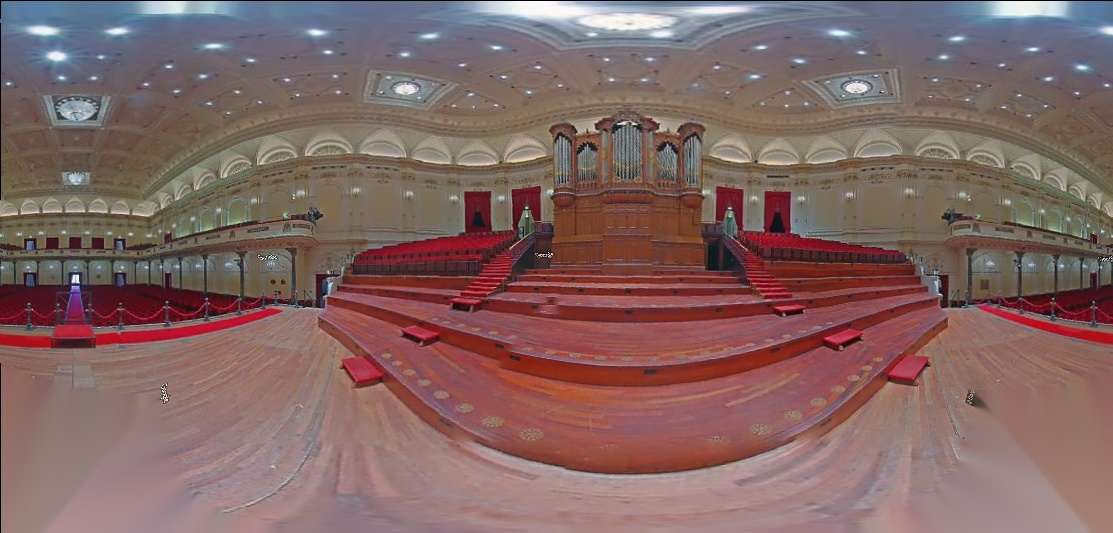
\includegraphics[width=5cm]{images/google_example/original}
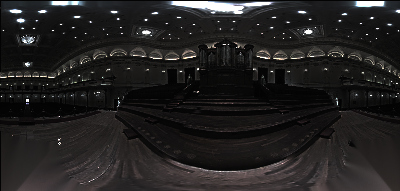
\includegraphics[width=5cm]{images/google_example/dark}
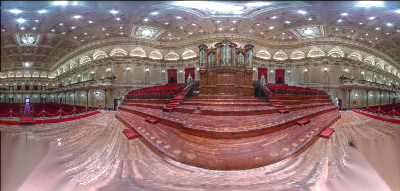
\includegraphics[width=5cm]{images/google_example/bright}
\caption{An example LDR panorama, with dark and light exposures extracted the predicted HDR environment.}\label{fig:google}
Source: Google
\end{figure}
\subsection{Bootstrapping Extra Light Probes}
A significant issue with generating the data is the lack of large datasets of HDRI environment maps. We initially used a dataset of 175 environment maps from HDRIHaven.com, an improvement over the 105 in \cite{RematasCVPR2016}. We found that our validation scores on unseen lighting continued to improve indicating that our model was not overfitting to the lighting scenarios presented. Qualitatively however it appeared that the model would primarily learn features from the training lightmaps and was at times effectively selecting the closest previously seen environment. This could be confirmed by training a model without the background present, which would perform significantly worse. While this may be effective at producing realistic lighting, the aim of this work is to encourage the model to learn how the reflectance of an object maps to the lighting conditions. To mitigate this behaviour and reduce overfitting to the environment we aimed to increase the size of our lighting dataset considerably. 
\newline
Collecting additional HDRI panoramas would be infeasible due to the lack of equipment and time and so we took the approach to producing HDR estimates from existing LDR content. The biggest available dataset of LDR panoramas is Google Street View \cite{GoogleMaps}, with both indoor and outdoor scenes. While this dataset is huge and provides a more realistic sample of lighting conditions, it is only available in low dynamic range. Fortunately, there is plenty of previous work in the area of converting LDR content to HDR, particularly using CNNS to find light sources and tonemap content. We make use of \cite{2018arXiv180302266M}, a very recent work that uses both a local and global branches to produce accurate tonemappng predictions. It is important to note that this network is intended as a general purpose image regressor, and is not trained on panoramas in particular. It would certainly be possible to improve results by retraining, or fine-tuning, the network on our existing set of HDR panoramas to produce better light probes. We make use of the image stitching and inpainting tools within OpenCV to create panoramas from different views on Google Street View, and use the aforementioned HDR-Expandnet to bolster our dataset with an additional 237 lightmaps. An example is shown in \ref{fig:google} Our models are trained both with and without these additions to find any issues with overfitting or malformed data produced by ExpandNet.
\begin{figure}[H]
\centering
\includegraphics[height=10cm]{images/Stereo}
\caption 
\newline
The first stereo image architecture. Weights are shared in the first 3 encode blocks, and the outputs are simply concatenated.
\label{basic}
\end{figure}
\section{Model Architecture}
\subsection{Siamese Layers}
To construct a model that produces good results, while minimising network size for performance and training times, it is important to carefully consider the problem being solved and the features and patterns that are being learned. By using stereo views we aim to find correspondance between similar features and an understanding of geometry due to the parallax effect. To this end we present results from a 'siamese' network, where the weights in the convolutional layers are shared, such that the same features are extracted from each view. The two inputs are fed into two identical 'Encode' blocks, consisting of a number of convolutional layers with batch normalization and max pooling. However, during the training process, only the weights for the first path are trained. These weights are duplicated in the second path to ensure that the same convolutions are being performed on each image of the pair. The output of these two paths is then concatenated before being passed into the deconvolutional steps, as shown in \ref{basic}. The output of the intermediate convolutions from the right branch is also kept for use as \textit{Multi-Scale} features, in more advanced architectures.
\subsection{Cosine Similarity Pyramid}
\begin{figure}[H]
\label{pyramid}
\centering
\includegraphics[width=14cm]{images/Pyramid}
\caption{The Cosine SImilarity Pyramid as implemented. Decode path removed for brevity.}
\end{figure}
We can further encourage the network to perform stereo matching by using the dot product technique as suggested in \cite{7780983}. After using shared weights to extract the same features from each image, we then perform a dot product operation on the L2-Normalised output to find the \textit{Cosine Similarity}
\[\bm{a}\cdot \bm{b} = \lvert a \rvert \lvert b\rvert \cos(\theta) \]
which represents the cosine of the angle between the two inputs. On a raw image, if two pixels are identical in value, they will have a cosine similarity of 1, and so we would find the nearest matching points from the values closest to 1. Instead of comparing raw pixels, we instead compare the intermediate representation, to find the similarity between features rather than pixels. The resultant correlations then represent the feature disparity maps. The correlation can then be concatenated with the original features before being passed as input to further convolutional layers, starting with a 1x1 convolution to act as a \textit{Fusion} layer.
\newline
A drawback of traditional block-disparity methods for stereo matching is that the block size significantly affects the accuracy of the calculated disparity. Larger block sizes have the important benefit of reliability, as it is easier to find unique matching blocks within the two images than it is to find matching pixels, for example. In our \textit{Cosine Similarity} step, we are effectively performing a block disparity on a spatially reduced representation of the image. Industry standard stereo matching methods deal with this by using a pyramid of block sizes, and fusing the results. To avoid suffering the same problems, we present a different model using a \textit{Cosine Similarity Pyramid}, where we perform our similarity step of each intermediate stereo output, as shown in \ref{pyramid}. This way, we can estimate similarity of features at different scales, exploting both the robustness of large blocks and the accuracy of small ones. Each similarity is concatenated to the stereo output as before. This method does present a significant performance comprimise, requiring more computation and memory to produce our full intermediate similarity representation.
\subsection{Other Features}
We experimented with different techniques for feature extraction that would benefit geometry and lighting understanding. Multi-scale features are also used, passing features for the second path into the deconvolutional layers. The model was trained with similar parameters to the previous network, using a L1 loss function on the predicted and ground truth environment map. For training we used a momentum optimizer with learning rate 1.7e-8
\newline
\todo{Dot product}
For our prediction task we make the following assumptions:
\begin{itemize}
\item Provided objects consist of a single material with constant albedo. Materials can contain Diffuse, Specular and Subsurface properties.
\item Geometry and lighting remain static between both stereo views.
\item Stereo view distance is kept constant, though object size can vary. Views are also parallel.
\item Subjects are modelled as floating objects. In the use-case where lighting on a surface is required, the surface lighting can be composited onto the light probe trivially.
\item Camera intrinsics are kept constant.
\end{itemize}

\section{Experiments}
To determine the best features for the task, we evaluated the performance of a suite of configurations:
\begin{itemize}
\item Dematerial model with known geometry.
\item Basic Concatenation model without shared weights.
\item Basic Concatenation model with shared weights.
\item Single Dot Product model.
\item Single Dot Product model without background data.
\item Single Dot Product model with augmented data.
\item Cosine Similarity Pyramid model.
\item Cosine Similarity Pyramid model with Multi-Scale features.
\end{itemize}
All models were trained for 100 epochs, with a learning rate of 1.7e-8, and evaluated on 1000 validation samples. A batch size of only 16 was used, due to memory requirements of the larger networks. We only quanititatively evaulate the quality of the lighting prediction, however surface normals are also produced as an output too all models aside from 'Dematerial'.
\chapter{Critical Evaluation}
\label{chap:evaluation}
\section{Experimental Results}
\subsection{Effect of Shared Weights}
\begin{figure}[H]
\newlength\figureheight
\newlength\figurewidth
\setlength\figureheight{6cm}
\setlength\figurewidth{12cm}
\centering
% This file was created by matplotlib2tikz v0.6.16.
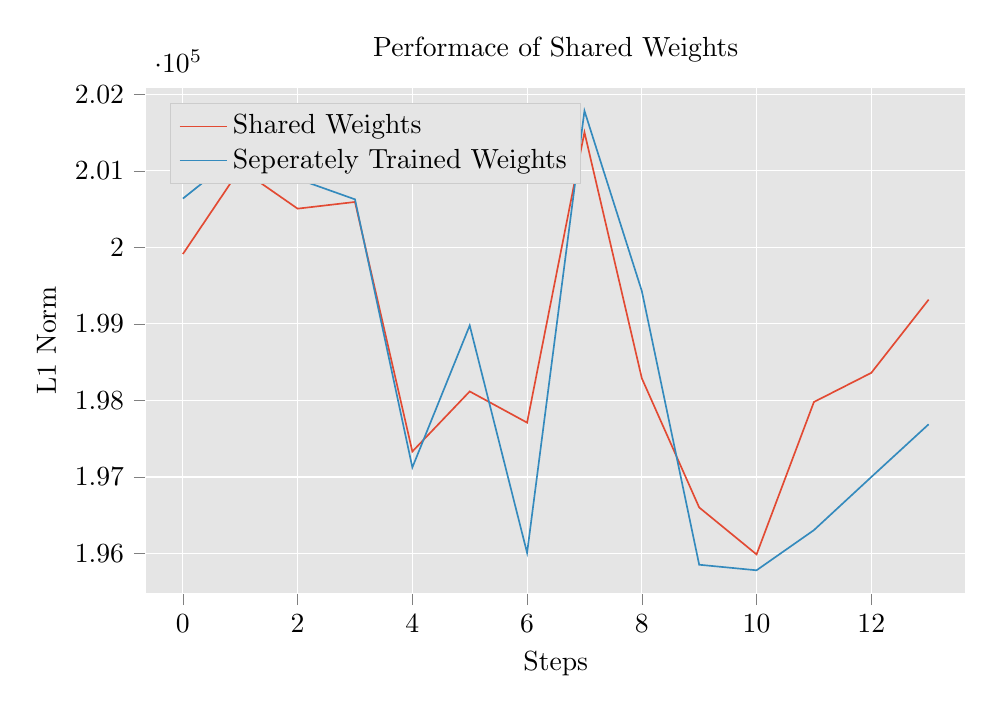
\begin{tikzpicture}

\definecolor{color1}{rgb}{0.203921568627451,0.541176470588235,0.741176470588235}
\definecolor{color0}{rgb}{0.886274509803922,0.290196078431373,0.2}

\begin{axis}[
title={Performace of Shared Weights},
xlabel={Steps},
ylabel={L1 Norm},
xmin=-0.65, xmax=13.65,
ymin=195480.29140625, ymax=202083.84921875,
width=12cm,
height=8cm,
tick align=outside,
tick pos=left,
xmajorgrids,
x grid style={white},
ymajorgrids,
y grid style={white},
axis line style={white},
axis background/.style={fill=white!89.80392156862746!black},
legend entries={{Shared Weights},{Seperately Trained Weights}},
legend style={at={(0.03,0.97)}, anchor=north west, draw=white!80.0!black, fill=white!89.80392156862746!black},
legend cell align={left}
]
\addlegendimage{no markers, color0}
\addlegendimage{no markers, color1}
\addplot [semithick, color0]
table {%
0 199912.765625
1 201026.984375
2 200505.734375
3 200593.0625
4 197332.296875
5 198117.484375
6 197710.078125
7 201504.21875
8 198289.265625
9 196601.453125
10 195987.859375
11 197979.546875
12 198360.421875
13 199317.171875
};
\addplot [semithick, color1]
table {%
0 200637.09375
1 201236.375
2 200893.953125
3 200627.1875
4 197124.421875
5 198979.375
6 196008.40625
7 201783.6875
8 199429.421875
9 195853.15625
10 195780.453125
11 196305.421875
12 196999.203125
13 197688.421875
};
\end{axis}

\end{tikzpicture}
\caption{L1 Norm between predictions and GT on validation set. Basic concatenation graph is used, with and without shared weights.}
\end{figure}
We found that using shared weights on our basic concatenation model had very little effect on the accuracy of results. In our training process we use the L1 norm loss to determine how to reweight our graph. For the siamese network, new weights are only calculated for the left branch, and then duplicated to the right branch. When the weights are trained seperately, they will eventually converge on, or even outperform the original weightings.
\subsection{Concatenation VS Dot Product}
\begin{figure}[H]
\setlength\figureheight{6cm}
\setlength\figurewidth{12cm}
\centering
% This file was created by matplotlib2tikz v0.6.16.
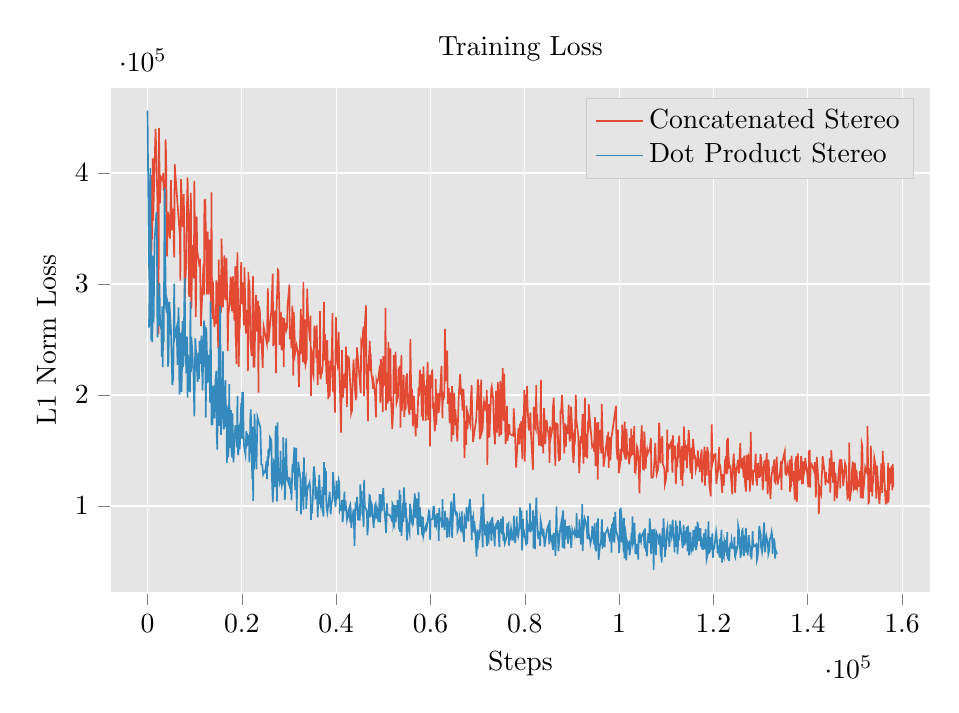
\begin{tikzpicture}

\definecolor{color1}{rgb}{0.203921568627451,0.541176470588235,0.741176470588235}
\definecolor{color0}{rgb}{0.886274509803922,0.290196078431373,0.2}

\begin{axis}[
title={Training Loss},
xlabel={Steps},
ylabel={L1 Norm Loss},
xmin=-7907.2, xmax=166051.2,
ymin=21681.686328125, ymax=476955.383984375,
width=12cm,
height=8cm,
tick align=outside,
tick pos=left,
xmajorgrids,
x grid style={white},
ymajorgrids,
y grid style={white},
axis line style={white},
axis background/.style={fill=white!89.80392156862746!black},
legend entries={{Concatenated Stereo},{Dot Product Stereo}},
legend style={draw=white!80.0!black, fill=white!89.80392156862746!black},
legend cell align={left}
]
\addlegendimage{no markers, color0}
\addlegendimage{no markers, color1}
\addplot [semithick, color0]
table {%
300 342090.4375
500 337827.875
700 398018.09375
800 323121.3125
900 350537.09375
1000 340310
1100 413261.28125
1200 357144.59375
1700 439710.5
1900 414285.90625
2000 392553.53125
2100 375877.09375
2332 254702.609375
2432 440334.5625
2632 372567.78125
2832 396522.5
3232 393363.53125
3332 400106.21875
3432 384254.40625
3532 389982.4375
3632 374218.65625
3732 365032.1875
3832 430330.6875
3932 416554.4375
4032 374277.25
4132 324805.46875
4332 364840.1875
4432 362166.59375
4532 349997.59375
4664 345549.8125
4764 340917
4964 393523.28125
5164 348388.125
5264 357072.65625
5464 367816.09375
5564 335902.75
5664 323941.96875
5764 407948.15625
6864 342757.40625
6964 303019.0625
7096 394352.625
7496 351207.15625
7696 381011.625
7896 286173.125
7996 303587.84375
8096 307943.15625
8196 318232.875
8296 356469
8496 395924.9375
8596 371138.625
8696 353564.1875
8796 290869.875
8896 288419.5625
8996 351285.25
9196 381999.59375
9296 277765.65625
9528 335035.25
9828 304917.8125
9928 392837.125
10228 270379.125
10328 296756.0625
10428 360747.75
10528 330566.46875
11028 315195.28125
11128 322734.6875
11328 262018.75
11860 317661.40625
11960 290380.71875
12060 375458.375
12260 375707.40625
12560 290593.4375
12760 347084.375
12860 327078.0625
12960 290541.90625
13160 339908.96875
13360 309428.375
13460 273875.21875
13560 382543.4375
13660 301848.9375
13760 268680.75
13860 302362.3125
14092 269267.59375
14192 261175.984375
14292 271052.0625
14492 263874.75
14592 303277.84375
14892 261222.28125
14992 242097.359375
15092 321948.3125
15192 273376.25
15292 274674.03125
15492 308033.53125
15592 274316
15692 340837.53125
15992 279041.84375
16192 309072.6875
16292 325727.9375
16424 295290.15625
16524 285528.96875
16724 323561.625
16924 283723.46875
17024 239858.8125
17124 272150.0625
17224 274829.75
17424 284292.8125
17524 296307.46875
17624 306655.65625
17724 286181.15625
17924 275778.1875
18024 304042.875
18124 306782.03125
18224 274021.6875
18324 277335.65625
18424 266954.625
18624 316000.96875
18656 254003.734375
18756 248440.1875
18856 227871.578125
19056 328389.9375
19256 271530.03125
19356 225349.890625
19456 264505.75
19556 263280.1875
19856 319741.28125
19956 282111.5625
20156 301477.5
20456 262641.34375
20556 315056.53125
20856 255292.0625
20956 276668.78125
21188 270302.3125
21288 221531.53125
21388 311027.625
21488 262047.15625
21588 303999.59375
21688 290108.8125
21788 249739.9375
22088 235159.796875
22288 290085.40625
22388 307115.40625
22488 224571.3125
22588 275318.9375
22688 224854.890625
22888 278904.375
22988 289987.5625
23088 257018.90625
23188 269137.6875
23420 284757.4375
23520 202198.515625
23620 280179.34375
23820 275741.6875
23920 263758
24020 246635.84375
24120 253322.9375
24420 224407.265625
24620 261716.296875
25320 246537.21875
25520 296055.28125
25652 247587.84375
26252 275980.3125
26552 309279
26652 243963.65625
26752 261411.6875
26952 245325.296875
27052 275967.8125
27252 219786.390625
27352 275441.46875
27652 312846.71875
27752 312320.3125
27952 276682
27984 244980.84375
28284 274879.375
28384 242725.65625
28484 240435.6875
28584 270403.71875
28684 246832.859375
28784 264979.40625
28884 225428.78125
28984 269314.75
29084 257952.59375
29184 265179.0625
29384 257811.1875
29584 261035.3125
29684 279346.09375
30084 299421.53125
30184 250417.890625
30316 258717.828125
30416 255591.796875
30516 241923.625
30716 280482.84375
30916 217519.125
31016 274775.375
31316 237830.828125
31616 244758.15625
31816 239811.65625
31916 237686.578125
32116 207050.453125
32216 228159.09375
32516 277584.53125
32616 237268.09375
32648 264440.3125
32848 270972.90625
32948 229705.1875
33048 301752.09375
33148 246775.453125
33248 238356.53125
33348 227887.484375
33448 268172.9375
33548 228258.671875
33748 232294.375
33848 295879.375
34048 269607.84375
34448 248484.515625
34548 271592.5
34648 199221.703125
34748 241170.046875
34948 237713.328125
34980 221578.640625
35180 217380.859375
35380 262536.6875
35580 252534.25
35680 258609.46875
35780 233015.421875
35880 262815.40625
36080 208979.078125
36180 240730.796875
36380 218691.921875
36480 222838.71875
36580 275449.6875
36680 214117.28125
36880 218999
36980 219896.09375
37180 227770.859375
37280 248506.359375
37312 254903.015625
37412 283900.125
37512 231165.328125
37612 254864.109375
38012 210065.84375
38112 249380.9375
38312 196248.953125
38412 230936.375
38612 198241.4375
38712 207368.3125
38912 230593.375
39012 231105.140625
39112 245565.265625
39212 273662.65625
39312 203037.890625
39412 226741.8125
39512 215251.3125
39744 184094.359375
39944 270397.71875
40144 237929.5
40344 227624.453125
40444 230506.90625
40544 256915.015625
40644 226437.90625
40844 200421.421875
41044 166132.34375
41244 240435.359375
41344 207295.765625
41444 197575.765625
41744 219150.1875
41944 206387.84375
42076 243499.0625
42176 213688.4375
42276 189345.453125
42376 235744.671875
42576 230369.53125
42676 234320.6875
42776 227362.78125
43076 201781.671875
43176 183287.234375
43376 186324.640625
43476 209486.640625
43676 231929.453125
43976 206318.75
44176 195284.171875
44276 233773.921875
44308 197170.125
44408 242884.140625
44708 228644.234375
45208 201691.140625
45308 246096.28125
45408 244125.453125
45808 261612.203125
45908 199060.296875
46008 256421.6875
46308 280824.0625
46408 229992.109375
46508 205005.765625
46608 209442.796875
46740 176485.09375
46840 226474.65625
46940 232509.859375
47140 248845.9375
47240 221753.515625
47340 237142.734375
47440 220637
47640 214673.328125
47840 205488.1875
47940 211138.125
48240 201724.75
48440 179898.984375
48540 212505.265625
48640 210666.40625
48940 214310.75
48972 216078.4375
49172 223330.59375
49272 221670.03125
49372 192959.328125
49472 232385.640625
49572 227953.015625
49772 219340.703125
49872 184677.078125
49972 235049.125
50272 208457.21875
50372 232996.578125
50472 278412.625
50572 186078.734375
50672 204466.53125
50772 199399.421875
50872 220100.84375
50972 192262.625
51072 247573.375
51304 194548.84375
51504 242041.8125
51604 198696.671875
51904 169368.109375
52104 189420.703125
52204 235913.625
52404 201045.421875
52604 238991.046875
52804 192850.796875
53104 198329.34375
53204 221889.9375
53304 220802.59375
53404 210527.625
53504 226414.75
53604 191663.125
53636 170652.28125
53736 217473.734375
53836 235880.984375
53936 185426.78125
54036 213554.078125
54136 210824.09375
54236 196051.96875
54336 218016.25
54436 180199.859375
54636 193729.6875
54736 186479.640625
54836 214387.359375
55036 219476.203125
55236 192700.78125
55536 182267.75
55636 203660.640625
55736 250237.203125
55968 186577.75
56068 205235.90625
56268 171914.390625
56368 176158.953125
56468 199740.03125
56868 162850.796875
56968 182507.4375
57168 170530.328125
57468 206285.59375
57568 199134.65625
57768 222649.75
58068 199461.046875
58168 180450.28125
58268 218723.5
58400 176923.109375
58500 225735.1875
58700 202362.59375
58800 208848.0625
58900 193353.015625
59000 176704.609375
59100 191127.4375
59400 229854.609375
59500 177543.359375
59700 190992.484375
59800 218127.171875
59900 153787.53125
60000 212579.953125
60400 222955.296875
60500 187784.90625
60600 193438.453125
60932 167243.046875
61032 180596.421875
61132 214361.34375
61232 173222.125
61332 183994.734375
61632 201832.296875
61732 184050.125
61932 192153.765625
62132 208895.140625
62332 226250.78125
62532 178903.09375
62632 202769.5625
62832 197393.546875
62932 198547.03125
63064 259487.109375
63264 212535.0625
63564 240055.375
63664 192094.546875
63864 206454.90625
64064 174662.84375
64164 202332.078125
64364 196008.140625
64464 157955.234375
64564 207970.171875
64764 186858.25
64864 163913.921875
64964 197241.625
65064 201559.46875
65164 172717
65264 187345.609375
65696 158276.046875
65996 199183.1875
66296 218895.328125
66496 199932.59375
66596 206039.625
66796 185900.84375
66996 205514.796875
67096 194883.953125
67196 143426.53125
67496 176940.03125
67596 155172.375
67628 190448.375
67728 184617.5
67828 169059.65625
68028 181366.859375
68428 173720.109375
68528 192223.40625
68728 209016.40625
68828 186337.0625
68928 177176.140625
69028 157707.78125
69428 169837.734375
69728 179214.9375
70060 214066.34375
70160 186398.671875
70260 196847.171875
70360 174093.75
70460 160045.125
70560 208954.625
70660 204120.9375
70760 213838.59375
70860 166208.140625
71060 169364.265625
71260 187289.53125
71360 193917.921875
71660 187647.84375
71760 188799.984375
71960 204699.609375
72060 137002.796875
72160 176635.75
72260 177592.28125
72292 179880
72392 191789.953125
72492 161653.875
72892 205564.28125
72992 207646.0625
73292 196307
73492 167371.640625
73692 155562.5625
73892 203600.640625
74092 166131.375
74292 211567.34375
74592 162504.28125
74624 188762.15625
74824 212715
74924 187235.9375
75024 164206.46875
75324 224283.3125
75524 176622.03125
75624 219248.1875
75924 155775.796875
76024 160539.734375
76224 189990.890625
76324 158789.875
76724 173618.390625
76824 164996.140625
77056 164310.359375
77556 163370.34375
77656 187961.03125
77956 161123.9375
78056 148441.390625
78156 134635.90625
78656 170418.90625
78756 157994.03125
78856 155532.375
78956 172664.390625
79156 171832.078125
79256 176503.578125
79288 163680.546875
79488 142054.8125
79588 177765.53125
79688 181158.84375
79788 172506.109375
79888 204616.75
79988 139971
80188 181669.5
80288 200254.90625
80388 192234.734375
80488 208301.28125
80588 189712.078125
80788 171768.578125
80888 168628.625
80988 168633.390625
81188 184371.859375
81288 167921.109375
81720 132603.203125
81920 189522.859375
82220 170578.625
82320 169330.21875
82420 208926.5625
82520 174046.4375
82620 182774.78125
82920 161647.4375
83020 154483.890625
83120 168036.359375
83220 154408.359375
83420 213706.0625
83520 154442.546875
83620 154162.75
83820 165015.25
83920 147469.921875
84052 188053.296875
84152 184701.625
84252 163081.578125
84352 155756.015625
84452 164820.703125
84552 176712.53125
84652 176541.015625
84852 167877.328125
84952 167070.71875
85152 159765.265625
85252 138848.390625
85352 171662.578125
85552 162704.53125
85852 169910.140625
85952 188095.6875
86152 197563.921875
86284 158740.609375
86484 136207.421875
86584 174638.03125
86984 173491.6875
87084 149461.53125
87284 140198.6875
87384 159792.546875
87484 141455.8125
87584 186114.65625
87684 183148.671875
87884 200097.265625
88284 164312.796875
88384 147492.8125
88484 174423.046875
88716 153419.921875
88816 172641.421875
89116 164910.453125
89316 191355.65625
89416 167770.03125
89516 158164.5625
89616 163380.109375
89716 160797.75
89816 189595.375
90016 172469.125
90116 151479.484375
90316 138617.875
90416 144823.265625
90516 168913.59375
90616 155354.0625
90816 200416.171875
90948 177392.5
91348 162960.828125
91548 129583.171875
91848 162856.203125
91948 157500.96875
92048 157367.046875
92248 182770.421875
92348 152945.40625
92448 138217.484375
92748 197694.3125
92848 144183.65625
92948 164321.609375
93148 162999.796875
93248 142758.59375
93380 176035.25
93480 166699.984375
93580 191661.734375
93780 178462.109375
93980 168926.875
94280 153528.046875
94580 155426.734375
94680 148950.90625
94880 179947.796875
94980 136064.21875
95080 149328.984375
95180 158807.40625
95280 175095.09375
95480 123755.0078125
95580 175655.46875
95612 147121.0625
95912 168521.875
96212 147505.21875
96312 191934.15625
96512 159063.125
96612 148301.84375
96712 135301.9375
97512 163678.234375
97612 144810.921875
97712 167096.859375
97812 134427.65625
97944 162145.765625
98144 141138.59375
98244 148979.484375
98344 160398.65625
99344 190124.6875
99444 153240.640625
99644 141735.890625
99744 168802.1875
99944 129430.171875
100244 138717.984375
100276 151387.421875
100376 140542.546875
100576 150702.828125
100676 173406.25
100776 152969.625
101076 147518.125
101176 176107.015625
101376 149016.421875
101476 141867.625
101576 169390.234375
101676 152385.625
101976 143850.953125
102176 137514.625
102276 161465.6875
102376 143236.875
102476 146463.28125
102576 169797.25
102608 145340.625
102708 148510.703125
102808 163896.953125
103008 146088.046875
103208 171990.734375
103308 129872.1875
103408 134082
103508 132106.296875
103808 153377.125
103908 151948.90625
104008 148460.03125
104108 137548.765625
104208 130079.171875
104308 111331.6015625
104508 147250.078125
104808 172603.078125
105040 133568.953125
105240 132913.25
105340 167038.859375
105440 160749.828125
105540 137401.296875
105640 133713
105740 144261.09375
105940 150216.484375
106040 146788.734375
106540 152273.34375
106740 161226.265625
106840 125529.828125
107240 126427.265625
107472 139249.859375
107672 156566.671875
107772 143192.3125
107972 128717.421875
108272 133347.78125
108372 157582.609375
108472 174962.390625
108572 170832.84375
108672 145026.109375
108772 138365.40625
108872 160629.578125
108972 149346.921875
109172 163021.09375
109272 137483.765625
109604 133499.5
109704 119498.4609375
109904 123279.484375
110104 132618.6875
110204 168722.5625
110304 130431.34375
110404 155146.953125
110704 152529.703125
110904 156326.453125
111104 158027.4375
111204 142418.9375
111304 130176.078125
111404 163682.6875
111604 146489.921875
111904 154288.875
111936 132564.25
112036 119763.90625
112136 133545.40625
112236 143320.5625
112336 134976.953125
112436 150415.53125
112536 148091.40625
112736 163330.96875
113136 123472.8828125
113236 145109.171875
113336 154099.078125
113436 117951.8828125
113536 140126.765625
113636 129816.546875
113736 171633.734375
113836 151072.71875
113936 159182.59375
114036 141146.0625
114236 146637.46875
114268 154847.984375
114368 133908.234375
114768 168278.5625
114968 150746.859375
115068 134143.109375
115168 129712.4375
115268 151133.5625
115368 151621.859375
115468 124188.0703125
115668 160386.671875
115868 150668.203125
115968 142029.0625
116068 145074.46875
116168 143844.921875
116268 132958.421875
116600 139305.625
116700 150136.96875
116800 139731.78125
116900 135188.34375
117000 142573.375
117100 130468.7734375
117300 143315.890625
117500 150872.625
117600 121072.375
117800 141241.09375
117900 135729
118100 153569.96875
118200 118338.078125
118300 149342.0625
118600 127461.8203125
118700 153067.25
118800 149773.109375
118900 147926.984375
118932 147528.296875
119132 119903.65625
119432 108733.46875
119632 173488.875
119832 138736.546875
120232 146489.484375
120432 146711.625
120632 119785.2421875
120732 124457.3203125
120832 126293
121232 153096.59375
121264 135655.65625
121364 137251.734375
121464 136469.59375
121864 111822.8359375
121964 128703.5390625
122164 118166.9765625
122264 123490.7578125
122464 142023.65625
122564 136964.484375
122664 144836.109375
122764 128445.25
122864 159897.046875
122964 129653.59375
123064 161372.703125
123164 148232.25
123364 134979.75
123596 135778.484375
123696 127669.40625
123896 116666.8671875
123996 110489.578125
124096 132642.6875
124296 147180.609375
124396 138276.53125
124496 137512.0625
124596 111867.6171875
124796 129192.03125
124896 132724.875
125096 137449.84375
125196 141599.9375
125396 129289.34375
125696 156641.015625
125796 140426.40625
125896 133637.625
125928 140226.5
126128 141595.828125
126428 125312.796875
126528 145481.921875
126728 118980.015625
126928 112956.5703125
127028 145024.59375
127228 145348.453125
127328 123249.484375
127428 137711.1875
127528 143388.1875
127628 141387.15625
127728 112986.4375
127928 166888.859375
128028 130218.5546875
128360 118723.203125
128460 131707.109375
128560 131389.5625
128760 131109.296875
128960 147071.046875
129060 122341.9765625
129160 132712.921875
129260 118372.1328125
129360 137800.171875
129460 137942.34375
129660 125399.546875
129760 133179.296875
129860 126378.96875
129960 146739.65625
130160 142036.65625
130460 114409.859375
130560 120881.2890625
130592 131232.171875
130792 140019.6875
130992 140797.53125
131092 122135.0625
131292 147933.890625
131492 110610.8671875
131592 122627.34375
131692 141722.515625
132092 106363.0546875
132292 125583.15625
132592 135887.46875
132692 130308.7734375
132892 142066.9375
132924 122603.765625
133124 121100.6875
133424 144558.828125
133624 119398.109375
133724 122218.015625
134124 130007.3125
134324 140664.5625
134424 114599.25
134524 137995.5625
135124 149176.171875
135256 128732.7890625
135456 128139.90625
135656 136352.46875
135756 134004.640625
136056 127891.421875
136156 141681.765625
136256 112775.5
136356 124338.0703125
136456 116965.0390625
136556 145399.671875
136856 121906.2421875
136956 131357.0625
137256 105873.7890625
137356 139137.21875
137456 141527.796875
137588 144771.46875
137688 103466.6328125
137788 113312.15625
137888 147404.25
138188 122934.953125
138288 133408.90625
138488 123703.515625
138588 144986.8125
138688 142145.046875
138788 119573.1328125
138888 124065.0546875
138988 119913.421875
139088 140211.40625
139188 129167.9296875
139388 133766.96875
139488 143235.015625
139688 133993.609375
139888 129791.359375
140120 117064.5625
140220 149985.53125
140320 119477.125
140420 150553.0625
140520 116628.46875
140620 138902.53125
140820 137809.109375
141320 131621.1875
141520 139444.3125
141720 107898.75
141920 144196.90625
142120 132065.03125
142252 123002.3046875
142352 92620.4375
142552 115973.734375
142852 111134
142952 125642.9921875
143052 132103.65625
143152 144963.8125
143652 127889.3828125
143752 118756.96875
143852 130576.6875
143952 123258.9140625
144352 121417.15625
144452 123088.15625
144684 142893.328125
144784 112010.3515625
144984 150211.03125
145384 120824.8359375
145484 126386.6484375
145584 139769.3125
145684 104315.484375
145784 124205.1484375
145884 129848.421875
146184 107025.671875
146484 125658.703125
146784 142072.328125
146884 115857.5546875
146916 124324.6953125
147016 131559.921875
147116 142146.171875
147316 133312.71875
147416 130698.546875
147516 117911.203125
147716 126425.734375
147916 138681.15625
148116 135742.046875
148416 107290.2734375
148516 107969.96875
148716 121349.3125
148816 157173.421875
148916 104262.84375
149248 116263.890625
149348 129774.4609375
149548 139943.328125
149748 114948.671875
149848 115667.1796875
149948 139111.8125
150048 136314.5625
150148 123957.90625
150248 114572.84375
150348 132597.703125
150548 117525.0625
150648 120104.453125
150848 122645.65625
150948 117290.921875
151048 131484.65625
151248 107153.421875
151448 156575.796875
151580 154352.28125
151680 106624.015625
151780 113658.6640625
151880 116743.3515625
152180 134687.015625
152280 133229.203125
152580 130055.9765625
152680 172161.65625
152880 102894.1015625
152980 103456.078125
153080 134192.5
153280 112819.765625
153380 154308.921875
153580 123155.59375
153680 108752.375
153780 120985.8125
153912 121426.421875
154012 130700.59375
154112 143395.75
154412 136017.625
154512 106584.9375
154712 136354.390625
155012 111046.1953125
155212 101845.7578125
155412 118947.75
155612 138495.28125
155712 124533.640625
155812 111831.40625
155912 149563.890625
156012 131845.234375
156112 139209.6875
156212 130458.0625
156244 125387.09375
156544 101371.53125
156644 113260.9765625
156844 113617.9453125
156944 102467.359375
157044 138778.890625
157144 103842.9921875
157344 134254.578125
157444 121025.375
157544 123078.609375
157644 128908.140625
157744 136163.375
157944 114149.5234375
158044 137699.5
158144 117203.75
};
\addplot [semithick, color1]
table {%
0 456261.125
300 318495.0625
500 284648.125
600 404469.0625
700 327573.6875
800 249309.109375
900 290008.59375
1000 287785.375
1100 325593.59375
1200 288333.625
300 260823.671875
400 287242.75
500 310582.4375
600 356390.65625
700 334921.75
800 301524.8125
900 271176.8125
1000 247624.125
1100 271377.40625
1300 268699.21875
1500 339434.6875
1900 364797.59375
2000 339271.5
2100 251986.578125
2200 272085.59375
2300 288227.34375
2333 284336.1875
2433 262314.4375
2533 300806.78125
2633 270628.34375
2733 263374.96875
2933 258858.890625
3033 234318.984375
3133 279885.875
3233 225139.75
3333 271128.09375
3433 247635.640625
3633 386613.375
3833 299328.125
3933 280266.625
4033 274214.375
4133 285788.0625
4233 283813.71875
4333 225686.640625
4433 230086.125
4533 253458.65625
4633 283766.125
4966 258808.75
5266 208851.53125
5466 215872.6875
5566 265040.375
5666 300250.84375
5766 251471.875
6166 260148.53125
6366 227113.171875
6566 278936.03125
6666 259351.96875
6766 200397.34375
6866 240350.203125
6966 256194.15625
7099 235338.6875
7199 202857.40625
7299 222529.0625
7399 266437.78125
7499 235560.96875
7599 225469.84375
7799 283455.625
7899 305204.625
7999 234935.609375
8099 253293.75
8199 219478.109375
8399 252264.34375
8499 197644.15625
8599 236346.0625
8899 205692.625
8999 202711.3125
9099 284327.28125
9199 220461.375
9299 252583.515625
9532 237432.953125
9632 225654.96875
9732 223564.25
9932 180673.90625
10132 251049.375
10532 218714.9375
10632 211757.078125
10732 238133.8125
10932 214374.0625
11032 248819.765625
11232 227973.53125
11432 253369.3125
11532 224253
11632 215531.96875
11665 204190.0625
11765 223729.5625
11965 266963.625
12065 225175.1875
12165 262997.75
12265 223082.703125
12365 179738.90625
12465 260864.78125
12765 211899
12865 212315.75
12965 236175.609375
13165 215123.515625
13265 193362.5625
13365 284111.84375
13565 172636.15625
13665 194925.921875
13765 173000.84375
13865 208132.453125
13965 203592.46875
14098 208411.734375
14198 178939.859375
14298 193340.90625
14398 213356.125
14598 221770
14698 161740
14798 150797.375
14898 211299.671875
14998 183011.53125
15098 243123.515625
15198 172234.46875
15398 280072.875
15598 164036.984375
15698 184253.6875
15798 198927.1875
15898 210831.65625
15998 239293.9375
16098 176658.734375
16198 168975.84375
16298 191679.21875
16331 183774.859375
16431 197285.65625
16531 213461.8125
16631 171286.90625
16731 190956.796875
16831 138655.03125
16931 188702.859375
17031 185219
17131 143911.09375
17231 161088.484375
17331 209812.3125
17431 152329.6875
17531 172501.140625
17731 186263.5625
17831 146809.109375
17931 143808.953125
18031 183424.203125
18131 146848.78125
18231 139273.203125
18531 166901.109375
18631 172032.4375
18764 172024.015625
18964 152827.15625
19064 199113.78125
19164 148197.3125
19264 145697.640625
19364 168425
19464 170467.1875
19564 151061.46875
19864 192849.1875
19964 160797.546875
20064 202762.78125
20164 179080.21875
20264 202613.53125
20364 165488.09375
20464 154244.21875
20764 146475.6875
20964 167591.0625
20997 155968.90625
21097 165726.59375
21197 155707.640625
21297 156584.875
21497 164207
21597 139381.4375
21697 153128.84375
21797 179326.21875
21897 186962.171875
21997 167866.78125
22097 152532.171875
22197 124169.15625
22297 171411.390625
22397 104694.921875
22497 163056.40625
22597 132946.875
22697 182994.84375
22797 164565.125
22897 150931.5
23097 133058.546875
23297 180190.75
23930 170536
24130 137467.421875
24330 137052.8125
24530 128237.53125
24830 130966.15625
24930 130768.234375
25230 140518.703125
25330 124273.203125
25430 144615.75
25530 135817.09375
25630 151429.40625
25663 142945.375
25863 150164.578125
25963 161783.28125
26263 159422.03125
26363 127230.359375
26563 103265.78125
26663 115948.9921875
26763 140588
26963 138781.796875
27063 116921.4375
27163 172200.15625
27263 132672.625
27363 125116.8515625
27463 104129.4296875
27563 175409.640625
27663 139552
27763 121922.828125
27863 134199.875
27996 119797.84375
28096 120961.28125
28196 149730.453125
28296 128670.6875
28496 118410.2890625
28696 122049.09375
28796 161901.015625
28896 136436.125
28996 143927.71875
29096 105466.828125
29196 111075.34375
29396 160853.828125
29496 137437.21875
29596 129140.5703125
29696 123665.21875
29996 119502.765625
30096 126236.8828125
30296 117385.875
30429 121351.9609375
30529 105223.71875
30729 137615.828125
30829 130307.359375
31129 152861.78125
31229 123406.984375
31329 114279.7109375
31529 152354.6875
31629 95630.203125
31729 116751.9921875
31829 125226.59375
31929 128482.484375
32029 139657.15625
32129 127375.84375
32229 130852.171875
32429 124532.046875
32529 92407.03125
32662 113647.4375
32862 109264.21875
32962 130767.8671875
33062 96654.8046875
33162 143825.78125
33262 108438.5546875
33362 120957
33562 124787.109375
33662 97556.25
33862 114148.1875
33962 114911.53125
34062 118513.9375
34262 119577.203125
34362 121123.828125
34462 117449.71875
34562 109232.96875
34662 87433.796875
34762 100051.09375
34862 93439.359375
34995 100807.875
35095 113634.203125
35195 129547.40625
35295 135599.03125
35495 125345.28125
35595 106822.9765625
35795 107236.6171875
35895 117389.6171875
35995 103118.984375
36095 89799.0625
36195 107255.359375
36295 101603.359375
36395 128108.234375
36695 102651.296875
36795 99395.8359375
36995 104808.9375
37095 117059.375
37195 95132.8359375
37295 90399.671875
37328 104728.296875
37428 139443.4375
37528 118763.5625
37628 134554.8125
37728 110099.78125
37828 131507.515625
37928 99921.09375
38028 96578.625
38128 94044.59375
38428 104835
38628 112799.578125
38828 92527.765625
39028 103121.171875
39128 104499.5703125
39228 106102.21875
39328 130399.671875
39528 117422.53125
39661 109434.3671875
39861 99183.75
39961 105819.1015625
40061 122756.9609375
40161 110056.65625
40261 111534.890625
40361 106816.359375
40561 122744.9140625
40661 120899.109375
40761 97132.1875
40861 98803.921875
40961 96892.890625
41061 96506.15625
41261 105512.046875
41361 85453.703125
41461 88915.890625
41761 112855.953125
41861 95739.71875
41994 104973.546875
42094 98752.265625
42294 87869.890625
42594 94978.4921875
42794 90612.8984375
42894 99855.59375
42994 101152.59375
43094 95835.6953125
43194 80388.5
43394 88317.390625
43694 96872.8828125
43894 64077.28125
43994 85802.546875
44094 100529.0078125
44294 98441.453125
44427 108180.984375
44527 100705.46875
44627 87202.109375
44927 99382.015625
45027 86835.359375
45127 119536.7421875
45227 104401.234375
45427 113313.0234375
45527 92774.7265625
45627 96739.4765625
45827 81171.140625
45927 123548.890625
46027 105018.828125
46127 98091.4375
46327 97752.3671875
46527 94386.140625
46627 73681.859375
46760 81617.453125
46860 90800.3359375
47060 109699.78125
47160 109326.9921875
47260 89965.6328125
47560 101488.46875
47660 100044.875
47760 90801.375
47860 85090.203125
47960 80327.3828125
48060 89635.359375
48160 89123.0546875
48260 101093.9296875
48360 102002.15625
48460 88802.921875
48560 93560.4453125
48660 96542.4375
48960 85536.5625
48993 98509.46875
49093 91870.4453125
49193 110761.4453125
49293 85391.28125
49393 92738.2265625
49493 96363.078125
49593 110493.765625
49693 95627.1875
49993 116095.8046875
50193 96673.234375
50293 94099.484375
50593 75670.078125
50793 102352.15625
50893 91972.953125
51093 92184.2578125
51293 92265.3828125
51426 91182.109375
51726 88734.96875
51826 86103.515625
51926 102303.015625
52026 101405.4921875
52126 83299.1640625
52226 85487.359375
52326 83870.9765625
52426 100740.7578125
52526 93228.6953125
52626 85253.546875
52726 92851.1875
52826 100635.7734375
52926 90196.8203125
53026 105170.390625
53126 96987.28125
53326 78896.328125
53426 114482.5078125
53526 76754.53125
53626 110240.1328125
53659 82701.0078125
53759 92777.734375
53859 73058.90625
54159 102629.15625
54259 85770.65625
54359 116731.0390625
54659 89523.15625
54759 103122.25
54959 73499.34375
55059 68974.15625
55159 84447.46875
55559 76045.125
55659 101959.609375
55859 95935.140625
55959 88089.71875
56092 85250.796875
56192 90457.015625
56292 82647.46875
56392 95324.3828125
56692 111259.09375
56792 89230.5234375
56892 94718.4375
57092 106859.84375
57192 84325.0390625
57392 73752.1796875
57492 112509.828125
57592 81389.953125
57692 95571.6015625
57792 98764.984375
57892 81300.078125
58092 91073.6796875
58192 75342.25
58325 73902.4140625
58425 89887.453125
58525 73925.109375
58625 76296.3125
59025 82069.8125
59125 79163.9921875
59225 80501.875
59625 93872.265625
59725 92141.328125
59825 93630.703125
59925 69472.4921875
60025 87971.4609375
60325 88005.3359375
60425 88189.703125
60625 99353.5859375
60758 99310.6953125
60958 80888.53125
61158 87328.5078125
61258 84182.0078125
61458 93457.828125
61558 88197.3515625
61658 87332.03125
61758 68684.4453125
61858 98016.0546875
61958 90112.0625
62258 86801.7265625
62358 84287.359375
62458 80623.96875
62558 106244.609375
62658 81756.3125
62758 84654.03125
62858 83575.8125
62991 78557.5
63091 95255.9296875
63191 87383.28125
63391 87198.4375
63491 71580.484375
63591 89681.34375
63691 86343.515625
63791 85805.765625
63891 80624.703125
63991 71975.921875
64391 104164.34375
64591 71250.21875
64691 84158.609375
64991 111388.984375
65191 95615.953125
65291 94100.90625
65324 94917.390625
65424 94687.171875
65624 93580.671875
65724 77428.546875
65824 78654.546875
66124 88810.09375
66224 83670.921875
66324 85615.765625
66424 81033.59375
66524 76375.140625
66624 95077.4453125
66724 84260.390625
67124 67695.140625
67224 89951.4921875
67424 86792.984375
67524 79568.7421875
67624 87486.65625
67657 98847.171875
67957 90645.4921875
68057 85938.4921875
68157 98618.8671875
68357 106459.921875
68557 93805.7109375
68757 69276.078125
68857 91111.515625
68957 86982.8125
69057 89323.4921875
69157 77280.0234375
69257 86432.515625
69357 75619.40625
69457 78686.59375
69557 73711.015625
69757 54339.7734375
69957 78876.1171875
69990 61407.734375
70190 77214.6640625
70290 69549.53125
70390 72938.140625
70490 76528.703125
70590 85465.1875
70690 85084.609375
70790 98971.75
70890 86206.890625
70990 73770.4296875
71090 62665.4140625
71190 111025.765625
71290 91953.9375
71590 73413.28125
71690 83326.7734375
71990 64001.5390625
72090 86307.8671875
72190 70325.453125
72323 68498.609375
72523 83719.578125
72723 85500.140625
72923 68703.2265625
73123 90252.828125
73223 79291.296875
73323 80618.296875
73523 71140.5625
73623 63627.2734375
73723 80797.34375
73923 83153.4375
74023 80262.828125
74223 81713.921875
74323 87312.296875
74423 75511.609375
74623 63052.859375
74656 85216.78125
74856 76106.625
74956 88463.21875
75156 74527.453125
75356 90590.625
75456 68553.6484375
75556 75660.828125
75756 66311.578125
76156 72152.78125
76256 83013.8828125
76356 82665.6015625
76556 84195.6640625
76656 64444.69921875
76756 76995.78125
76856 69125.5703125
77089 79160.984375
77289 71869.953125
77389 73475.8203125
77489 69075.84375
77589 73419.796875
77689 91225.8125
77789 73162.4453125
77889 67635.609375
77989 67527.6796875
78189 79537.0390625
78289 90624.109375
78389 76363.1640625
78489 74308.8203125
78589 72438.4375
78689 74961.609375
78889 84162.109375
78989 98837.9921875
79089 79024.609375
79189 83123.34375
79289 95914.234375
79422 60130.29296875
79522 72398.40625
79622 88493.09375
79722 77328.3125
79822 77620.140625
79922 72679.1875
80022 72681.1796875
80322 64505.41015625
80422 96093.5859375
80522 65813.5
80622 77702.71875
80922 83392.828125
81022 77089.3828125
81122 102449.921875
81222 76261.9140625
81322 80739.65625
81622 85692.65625
81655 78071.7109375
81755 96138.390625
81855 61922.62109375
82055 90928.640625
82155 61080.171875
82255 84686.546875
82455 107714.3828125
82555 89712.8203125
82755 76621.40625
82855 71320
82955 71657.390625
83055 77036.078125
83155 70041.09375
83255 64128.9921875
83355 87183.171875
83555 82591.296875
83655 74833.796875
83855 73256.921875
83955 79499.4140625
83988 77766.9765625
84188 63289.7421875
84488 72650.4140625
84588 76156.0234375
84788 80041.828125
84988 82365.515625
85088 76152.8046875
85188 65369.83984375
85288 87329.5234375
85388 68937.734375
85688 72071
85788 67742.125
85988 60435.82421875
86088 71613.15625
86188 70061.203125
86288 75870.59375
86321 71392.203125
86521 55180.95703125
86721 99770.890625
86821 73749.46875
86921 78081.875
87021 71798.265625
87121 59194.76171875
87421 74859.09375
87521 79987.03125
87821 87113.90625
88021 62271.63671875
88121 96136.46875
88221 78006.640625
88321 84361.765625
88421 61707.08984375
88521 87698.296875
88621 69772.140625
88654 75404.5625
88754 81519.859375
88954 72940.6015625
89054 81930.6953125
89154 66139.78125
89254 70566.6171875
89454 82414.03125
89654 74644.734375
89854 62322.171875
90054 78450.46875
90254 74898.3125
90454 74851.6640625
90554 77036.1484375
90654 73354.703125
90754 74704.53125
90954 77217.84375
90987 93754.3984375
91087 71723.8125
91387 72025.625
91487 75698.828125
91587 87995.375
91787 74937.2265625
91887 65368.73046875
92087 77737.125
92187 101661.921875
92287 59566.1171875
92387 75319.109375
92487 79395.890625
92687 88770.171875
92987 84605.140625
93187 77216.890625
93287 70102.078125
93320 76318.796875
93420 90992.890625
93520 74358.7109375
93620 74223.578125
93720 70469.25
93820 70247.546875
93920 66116.515625
94120 70186.4375
94220 74448.75
94320 82061.0625
94620 68488.203125
94720 65271.31640625
94820 84376.171875
94920 61480.73828125
95020 65068.6171875
95120 59125.78125
95220 67030.0625
95320 85380.265625
95420 74976.1171875
95520 88850.671875
95653 51474.04296875
95953 65224.84375
96153 66920.1875
96253 79067.6796875
96353 87973.109375
96453 61666.4375
96653 76852.734375
96853 65643.8359375
96953 62987.07421875
97053 74722.53125
97553 79517.4140625
97986 70083.578125
98086 71344.1484375
98286 79679.21875
98386 58095.0625
98486 83725.96875
98586 67963.984375
98686 81039.2421875
98786 79512.71875
98886 89910.25
98986 67104.421875
99086 74068.796875
99186 94778.9375
99286 81575.171875
99386 76633.359375
99486 76183.3203125
99786 70243.3125
99886 73227.2265625
99986 57538.125
100086 63260.28125
100186 97437
100286 67419.0078125
100319 98554.890625
100619 85746.375
100719 67260.828125
100819 81960.546875
100919 58914.48046875
101019 89215.296875
101119 52861.328125
101219 75183.9296875
101319 77848.7421875
101419 74928.90625
101519 51013.9765625
101719 67483.0078125
101919 63934.90625
102019 66849.2421875
102119 67437.4921875
102219 55551.08203125
102519 66040.4609375
102619 75202.453125
102652 75210.640625
102752 70737.4140625
102852 90640.4375
102952 66382.0546875
103152 70194.125
103252 84714.90625
103452 56445.4765625
103752 65899.3359375
103852 56929.10546875
103952 64516.765625
104052 51831.9140625
104152 74080.5
104252 66496.65625
104352 76068.484375
104452 72973.0234375
104652 68648.453125
104752 72824.7578125
105185 76538.296875
105285 69435.78125
105385 61804.609375
105485 79751.90625
105585 67911.8359375
105685 58949.703125
105785 65515.94921875
105885 54707.56640625
106185 75496.5625
106385 66684.4921875
106485 88768.984375
106685 76352.4140625
106785 56736.36328125
106985 72224.953125
107085 78954.109375
107185 71583.0625
107285 66163.546875
107318 42375.9453125
107418 79172.6953125
107518 74035.3203125
107618 68454.6484375
107818 55717.0390625
107918 75827.5390625
108318 70679.453125
108418 65303.2109375
108618 75335.5234375
108818 54707.1484375
108918 73123.375
109018 49101.46875
109118 68755.90625
109218 80326.53125
109318 63197.28125
109418 88838.7890625
109618 67606.03125
109751 54166.79296875
109851 70719.4765625
109951 60827.66015625
110051 76621.3828125
110251 81067.28125
110351 71402.90625
110551 68620.734375
110651 63166.9921875
110751 69176.921875
110851 83318.7421875
110951 76867.1328125
111051 76431.125
111151 73019.765625
111251 76799.140625
111351 87699.34375
111451 76427.4765625
111651 69461.7734375
111751 58244.9765625
111851 74020.78125
111951 65846.078125
111984 86970.3046875
112084 74491.2890625
112184 63183.0703125
112284 82364.125
112384 56601.8203125
112484 64840.49609375
112584 72845.0703125
112684 69421.859375
112884 86837.421875
112984 81827.03125
113084 79321.015625
113484 62156.30078125
113684 83029.7109375
113784 64552.3125
113884 67843.7734375
113984 77574.1171875
114084 68419.9296875
114184 69804.5859375
114317 80993.890625
114517 59142.640625
114617 82223.0546875
114717 70177.6796875
114817 55616.71484375
114917 62713.73828125
115117 76653.953125
115317 60111.171875
115417 61598.4921875
115517 67814.6796875
115617 59203.6015625
115717 78545.3515625
115817 63197.23828125
116017 65506.3359375
116117 75366.5390625
116217 81681.1328125
116317 60306.7421875
116517 65958.5
116617 85982.84375
116750 74541.1171875
116850 77207.1875
116950 68369.203125
117250 80042.921875
117350 64452.75390625
117450 63511.0546875
117550 69751.171875
117650 68614.078125
117850 60505.89453125
117950 75211.0390625
118150 61236.3515625
118350 79302.21875
118550 52014.171875
118750 55879.3203125
118950 86197.5859375
119083 58115.02734375
119283 59078.9375
119383 72111.671875
119483 60508.8515625
119783 75474.25
119883 53377.83984375
119983 61801.3125
120083 63036.7109375
120183 62560.0234375
120583 76834.828125
120683 73703.734375
120883 57434.84375
120983 61769.1171875
121183 58093.6484375
121283 54310.69140625
121316 70365.1484375
121416 53309.1796875
121516 62039.4765625
121616 71500.265625
121716 78480.5703125
121816 49035.64453125
122016 67929.21875
122116 54758.62109375
122216 53664.328125
122316 68189.40625
122416 66148.3359375
122616 58374.48046875
122716 69302.46875
122816 54784.015625
122916 76435.25
123016 51988.265625
123116 62406.0390625
123216 58846.078125
123316 50309.48828125
123516 63197.85546875
123616 66947.4609375
123649 63992.1953125
123749 63275.375
123849 68935.5
124049 62854.25
124349 61283.34375
124449 72499.4453125
124549 54716.5078125
124649 53627.5625
124749 63903.0546875
124849 58600.7265625
125149 64251.765625
125249 82189
125449 77431.265625
125649 61997.859375
125749 53284.08984375
125849 72099.96875
125949 68124.546875
125982 55557.09375
126082 78446.03125
126182 78971.7421875
126282 70182.53125
126382 73325.09375
126482 54786.484375
126582 66439.015625
126682 64055.359375
126882 80202.765625
127082 58041.5625
127182 61756.3984375
127282 55576.48046875
127482 73764.78125
127682 64910.1640625
127782 62659.26953125
127882 54254.24609375
127982 64017.8359375
128082 51920.359375
128182 61770.19921875
128315 77344.5
128415 64332.5625
128515 65466.08984375
128615 63716.0234375
128815 63935.7890625
129115 65559.7890625
129215 51041.9609375
129315 52702.24609375
129515 59335.03125
129715 82030.75
129815 78894.328125
129915 76849.3125
130015 75145.4140625
130115 62280.78125
130215 61227.765625
130315 58517.3125
130415 62082.23046875
130748 85301.40625
130848 69173.6015625
130948 58228.03125
131248 72159.0625
131348 69943.6328125
131548 67028.921875
131648 56602.19140625
131848 59745
131948 70918.859375
132048 71055.96875
132148 71457.7265625
132348 76599.1171875
132448 73339.140625
132548 56833.4375
132648 67582.1328125
132848 69540.4453125
132981 67478.4296875
133081 52543.9375
133181 60480.1640625
133481 56593.95703125
};
\end{axis}

\end{tikzpicture}
\caption{L1 Norm between predictions and GT on validation set. In the first version, the outputs from the siamese layers are concatenated, in the other they are normalised and the dot product is performed.}
\end{figure}
The dot product step results in a small improvement in accuraccy and a significant improvement in training speed. The dot product step is effectively a manually calculated similarity measure between the two views, and so the model can converge on the depth features earlier in the training process. We believe that the performance difference is minimal as the model is already very deep, and training would likely converge on the depth features eventually. As a result we also show the effect with a much shallower model. \todo{Show this}

\subsection{Effect of Background}
\begin{figure}[H]
\setlength\figureheight{6cm}
\setlength\figurewidth{12cm}
\centering
% This file was created by matplotlib2tikz v0.6.16.
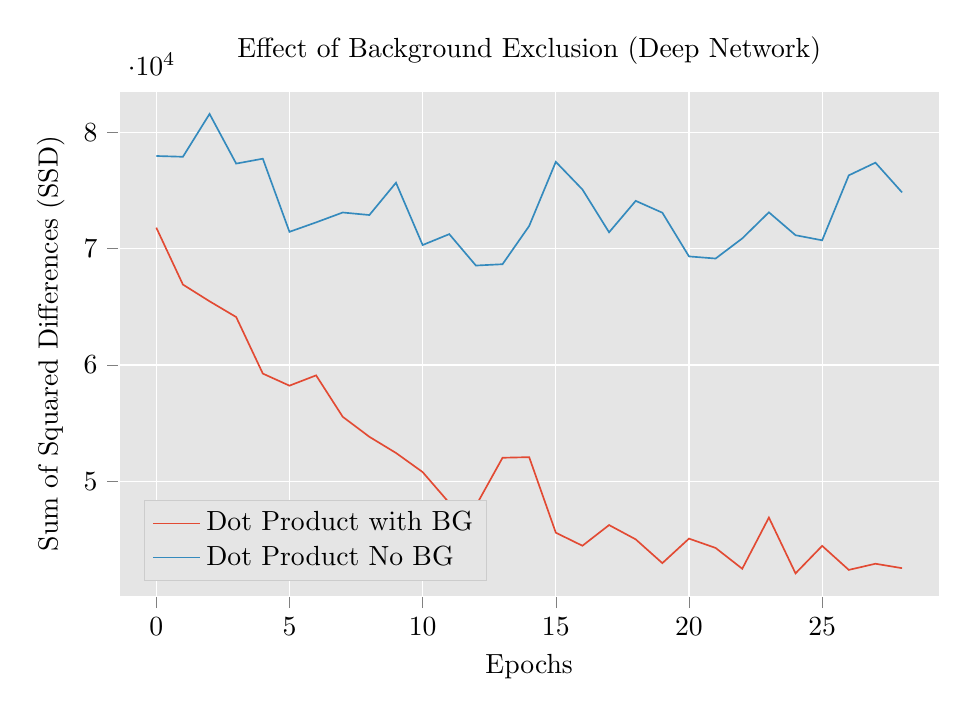
\begin{tikzpicture}

\definecolor{color1}{rgb}{0.203921568627451,0.541176470588235,0.741176470588235}
\definecolor{color0}{rgb}{0.886274509803922,0.290196078431373,0.2}

\begin{axis}[
title={Effect of Background Exclusion (Deep Network)},
xlabel={Epochs},
ylabel={Sum of Squared Differences (SSD)},
xmin=-1.4, xmax=29.4,
ymin=40089.8203125, ymax=83578.8359375,
width=12cm,
height=8cm,
tick align=outside,
tick pos=left,
xmajorgrids,
x grid style={white},
ymajorgrids,
y grid style={white},
axis line style={white},
axis background/.style={fill=white!89.80392156862746!black},
legend style={at={(0.03,0.03)}, anchor=south west, draw=white!80.0!black, fill=white!89.80392156862746!black},
legend cell align={left},
legend entries={{Dot Product with BG},{Dot Product No BG}}
]
\addlegendimage{no markers, color0}
\addlegendimage{no markers, color1}
\addplot [semithick, color0]
table {%
0 71815.9140625
1 66918.078125
2 65479.265625
3 64121.98046875
4 59256.625
5 58217.87890625
6 59104.46875
7 55539.98828125
8 53817.453125
9 52427.26953125
10 50782.52734375
11 48130.453125
12 47883.140625
13 52014.94921875
14 52066.69140625
15 45566.328125
16 44443.25390625
17 46223.32421875
18 44993.12890625
19 42946.69140625
20 45057.19140625
21 44253.609375
22 42463.171875
23 46869.61328125
24 42066.59375
25 44432.17578125
26 42364.625
27 42895.50390625
28 42513.109375
};
\addplot [semithick, color1]
table {%
0 77981.546875
1 77914.5078125
2 81602.0625
3 77327.15625
4 77749.1640625
5 71455.625
6 72268.7109375
7 73119.2734375
8 72902.3203125
9 75683.4921875
10 70319.9375
11 71257.7265625
12 68554.953125
13 68669.1015625
14 71960.2578125
15 77478.421875
16 75098.2890625
17 71414.4453125
18 74120.765625
19 73100.7265625
20 69340.5390625
21 69158.5390625
22 70889.375
23 73134.9296875
24 71164.2421875
25 70725.546875
26 76315.390625
27 77407.84375
28 74847.6796875
};
\end{axis}

\end{tikzpicture}
\caption{Comparison of L1 Norm accuracy with and without the background present. Lighting effects on the subject remain the same.}
\end{figure}
The model is able to infer much of the lighting without the background, indicating that it is learning the lighting conditions from the subject. However, adding the background improves the performance significantly. The background not only gives an indication of the physical environment the subject inhabits, but also the colors and intensities to expect. This data, in theory, should make it easier to determine the difference between reflectance, albedo and shadows on the subject as well as indicate the hue of the resulting environment map. Ou results indicate that the background information is useful for estimating the lighting accurately.
\subsection{Cosine Similarity Pyramid}
\begin{figure}[H]
\setlength\figureheight{6cm}
\setlength\figurewidth{12cm}
\centering
% This file was created by matplotlib2tikz v0.6.16.
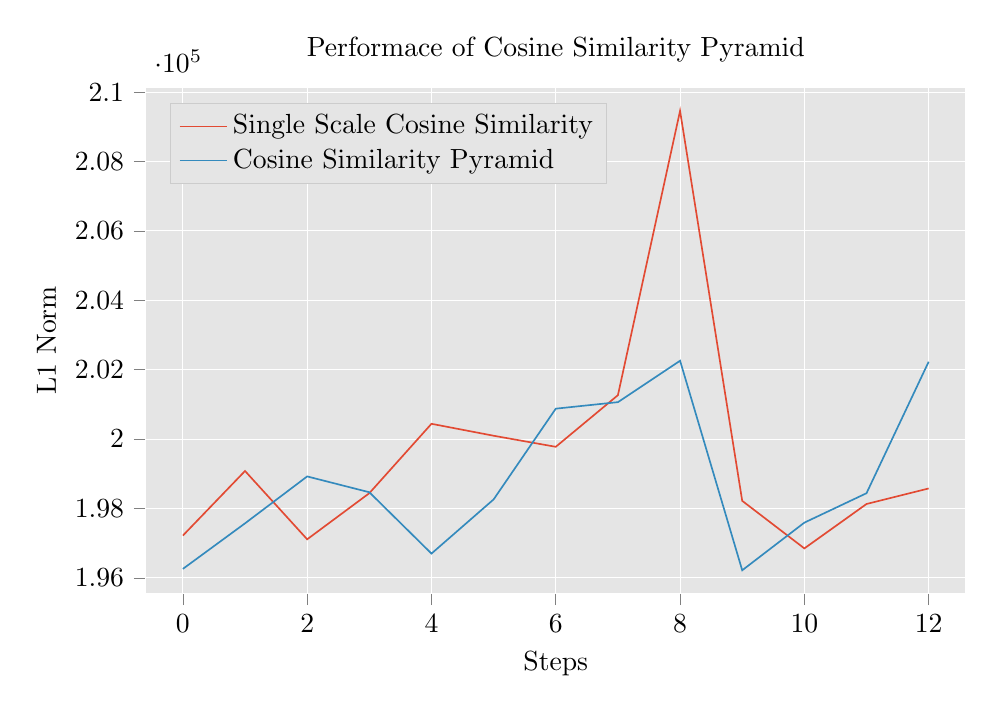
\begin{tikzpicture}

\definecolor{color1}{rgb}{0.203921568627451,0.541176470588235,0.741176470588235}
\definecolor{color0}{rgb}{0.886274509803922,0.290196078431373,0.2}

\begin{axis}[
title={Performace of Cosine Similarity Pyramid},
xlabel={Steps},
ylabel={L1 Norm},
xmin=-0.6, xmax=12.6,
ymin=195555.86015625, ymax=210121.56171875,
width=12cm,
height=8cm,
tick align=outside,
tick pos=left,
xmajorgrids,
x grid style={white},
ymajorgrids,
y grid style={white},
axis line style={white},
axis background/.style={fill=white!89.80392156862746!black},
legend entries={{Single Scale Cosine Similarity},{Cosine Similarity Pyramid}},
legend style={at={(0.03,0.97)}, anchor=north west, draw=white!80.0!black, fill=white!89.80392156862746!black},
legend cell align={left}
]
\addlegendimage{no markers, color0}
\addlegendimage{no markers, color1}
\addplot [semithick, color0]
table {%
0 197218.3125
1 199080.0625
2 197110.71875
3 198440.03125
4 200439.765625
5 200095.78125
6 199776.78125
7 201264.515625
8 209459.484375
9 198219.90625
10 196848.78125
11 198128.296875
12 198576.578125
};
\addplot [semithick, color1]
table {%
0 196258.0625
1 197571.0625
2 198923.0625
3 198467.046875
4 196699.53125
5 198260.65625
6 200876.03125
7 201064.0625
8 202257.921875
9 196217.9375
10 197591.296875
11 198439.125
12 202228.28125
};
\end{axis}

\end{tikzpicture}
\caption{Comparison of model with single Similarity layer, and model with a pyramid of similarity measurements.}
\end{figure}

\subsection{Effect of Multi-Scale Features}
\begin{figure}[H]
\setlength\figureheight{6cm}
\setlength\figurewidth{12cm}
\centering
% This file was created by matplotlib2tikz v0.6.16.
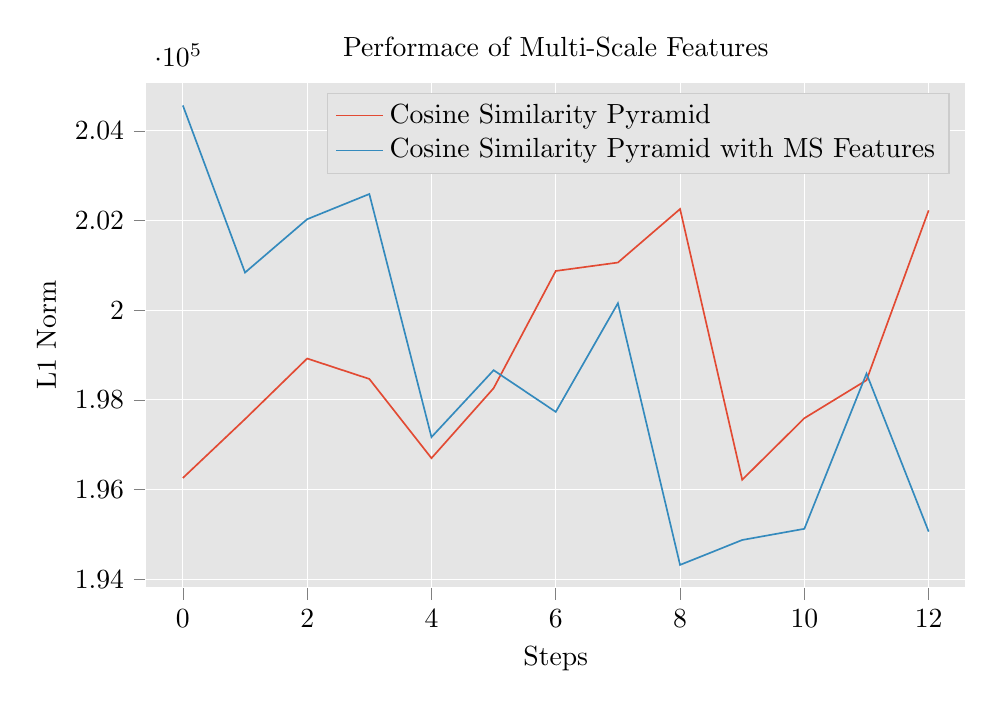
\begin{tikzpicture}

\definecolor{color1}{rgb}{0.203921568627451,0.541176470588235,0.741176470588235}
\definecolor{color0}{rgb}{0.886274509803922,0.290196078431373,0.2}

\begin{axis}[
title={Performace of Multi-Scale Features},
xlabel={Steps},
ylabel={L1 Norm},
xmin=-0.6, xmax=12.6,
ymin=193805.93828125, ymax=205080.57734375,
width=12cm,
height=8cm,
tick align=outside,
tick pos=left,
xmajorgrids,
x grid style={white},
ymajorgrids,
y grid style={white},
axis line style={white},
axis background/.style={fill=white!89.80392156862746!black},
legend style={draw=white!80.0!black, fill=white!89.80392156862746!black},
legend entries={{Cosine Similarity Pyramid},{Cosine Similarity Pyramid with MS Features}},
legend cell align={left}
]
\addlegendimage{no markers, color0}
\addlegendimage{no markers, color1}
\addplot [semithick, color0]
table {%
0 196258.0625
1 197571.0625
2 198923.0625
3 198467.046875
4 196699.53125
5 198260.65625
6 200876.03125
7 201064.0625
8 202257.921875
9 196217.9375
10 197591.296875
11 198439.125
12 202228.28125
};
\addplot [semithick, color1]
table {%
0 204568.09375
1 200840.40625
2 202030.71875
3 202592.6875
4 197169.65625
5 198661.828125
6 197732.484375
7 200156.921875
8 194318.421875
9 194874.515625
10 195123.984375
11 198586.671875
12 195061.6875
};
\end{axis}

\end{tikzpicture}
\caption{Comparison of model with single Similarity layer, and model with a pyramid of similarity measurements.}
\end{figure}
Multi-Scale features aim to improve performance by making use of convolutional features at a range of scales. Between each encode block, the output is both passed to the next encode layer, and the corresponding decode layer with the same feature size. This results in faster training as the model can make useful predictions early on before a deeper understanding, that makes use of all the layers is built.
\section{Final Model Accuracy}
To evaluate the accuracy of the models we use a suite of image comparison measures on the produced HDRI environment maps. It is essential that the metrics used suitably evaulate the image similarity, and so we consider which image properties are most influential of the resulting lighting. The most basic estimation should be able to capture the direction and intensity of direct lights within the scene. Often there are few direct lights, but their effect on lighting dominates the overall scene illumination. Better predictions will be able to capture some information on indirect lighting, such as sky or wall colour and brightness.
\todo{Talk a bit more about this}
\newline 
We start with two basic difference metrics, the L1 and L2 norm, which are both per-pixel Minkowski distances. These measures are fast to calculate and simple to implement and so are often used as the loss function in image regression tasks. L2 norm involves the squaring of pixel differences, and exagerrates the effect of large pixel differences on the overall similarity score. In the HDR domain this can mean that direct lights, such as the sun, which are predicted to be in a slightly different direction, will have a severe impact on the similarity, despite having a minor effect on the resulting illumination. When we inspect light sources in sRGB photographs, it appears as if the light source is large and emmitting light from a radius, as the higher brightness values fall outside of the cameras exposure bracket. \ref{rgb_example} demonstrates this effect, as parts of the woman's face, as well as the surrounding sky have the same colour values as the center of the sun, as the camera fails to capture the brightness rage. A minor misprediction in sun position here will have little effect on the L2 distance, but in HDR would have a significant impact.
\newline
Another commonly used image comparison metric is the SSIM \cite{1284395},
\[SSIM(x,y) = \frac{(2u_xu_y + c_1)(2\sigma_{xy} + c_2)}{(u^2_x + u^2_y + c_1)(\sigma^2_x + \sigma^2_y + c_2)}\]
which aims to predict the accuracy of an image with human perception. It is a measure of structure, which takes luminance and contrast into account, and so is better suited for HDR. Finally, we assess the models ability to identify the direction of the provailing light source, by taking the distance between the brightest pixel in the ground truth and predicted image. For assessment we use a validation set of 1000 images, under new environment maps and models with random materials and rotations.
\newline
On our synthetic benchmark, our deep stereo model achieved a Mean Squared Error of 150.03, with the 50th and 75th percentile being 2.67 and 8.3 respectively. This implies that while the model performs well in most tested scenarios, there are some cases where the predictions are vastly incorrect, as shown in \ref{ssim_results}. For the SSIM test, the stereo model achieves a respectable average of 0.322, with 50th and 75th percentiles of 0.30 and 0.41. These results are close to that of the previous work that relied on known surface geometry.
\newline
Our method does not achieve the accuracy of the original 'What is around the camera?' work. However an important factor to consider is that the original work made use of known surface geometry, making the input sparse reflectance map a better representation of the light on the object. If noisy, estimated surface normals are used, as suggested by the original authors, our work provides more complete estimates. Furthermore, the differences in training data between the original work and ours have a significant impact on the resulting accuracies. The original model was trained on classes from the Shapenet 'Car' class, mostly consisting of curved objects. This means that the image contains more surface normals to estimate light from, and can build a denser reflectance map. The original work also only contained materials from the MERL BRDF dataset, capturing 100 different common materials. Our material range is more complete, using materials generated from BSDF shader parameters.
\todo{Put a table of results here followed by discussion}
\begin{figure}[H]
\centering
\begin{tabular}{ |p{3cm}||p{3cm}|p{3cm}|p{3cm}|p{3cm}|  }
 \hline
 \multicolumn{5}{|c|}{SSIM Evaluation} \\
 \hline
  & Input Data &Ground Truth Environment&Predicted Environment&SSIM Score\\
 \hline
 25th Percentile(Synth)&\parbox[c]{1em}{
 \includegraphics[width=2cm,trim=-10 0 0 -10]{images/deep_stereo/25p_ssim_input}}&\parbox[c]{1em}{\includegraphics[width=2cm,trim=-10 0 0 -10]{images/deep_stereo/25p_ssim_gt_tm}}&
\parbox[c]{1em}{\includegraphics[width=2cm,trim=-10 0 0 -10]{images/deep_stereo/25p_ssim_pred_tm}}& 0.22\\
 50th Percentile(Synth)&\parbox[c]{1em}{
 \includegraphics[width=2cm,trim=-10 0 0 -10]{images/deep_stereo/50p_ssim_input}}&\parbox[c]{1em}{\includegraphics[width=2cm,trim=-10 0 0 -10]{images/deep_stereo/50p_ssim_gt_tm}}&
\parbox[c]{1em}{\includegraphics[width=2cm,trim=-10 0 0 -10]{images/deep_stereo/50p_ssim_pred_tm}}& 0.30\\
 75th Percentile(Synth)&\parbox[c]{1em}{
 \includegraphics[width=2cm,trim=-10 0 0 -10]{images/deep_stereo/75p_ssim_input}}&\parbox[c]{1em}{\includegraphics[width=2cm,trim=-10 0 0 -10]{images/deep_stereo/75p_ssim_gt_tm}}&
\parbox[c]{1em}{\includegraphics[width=2cm,trim=-10 0 0 -10]{images/deep_stereo/75p_ssim_pred_tm}}& 0.41\\

 \hline
\end{tabular}

\label{ssim_results}
\caption{Demonstration on test set.}

\end{figure}

\begin{figure}[H]
\centering
\begin{tabular}{ |p{3cm}||p{3cm}|p{3cm}|p{3cm}|p{3cm}|  }
 \hline
 \multicolumn{5}{|c|}{MSE Evaluation} \\
 \hline
  & Input Data &Ground Truth Environment&Predicted Environment&MSE Score\\
 \hline
 25th Percentile(Synth)&\parbox[c]{1em}{
 \includegraphics[width=2cm,trim=-10 0 0 -10]{images/deep_stereo/25p_mse_input}}&\parbox[c]{1em}{\includegraphics[width=2cm,trim=-10 0 0 -10]{images/deep_stereo/25p_mse_gt_tm}}&
\parbox[c]{1em}{\includegraphics[width=2cm,trim=-10 0 0 -10]{images/deep_stereo/25p_mse_pred_tm}}& 0.22\\
 50th Percentile(Synth)&\parbox[c]{1em}{
 \includegraphics[width=2cm,trim=-10 0 0 -10]{images/deep_stereo/50p_mse_input}}&\parbox[c]{1em}{\includegraphics[width=2cm,trim=-10 0 0 -10]{images/deep_stereo/50p_mse_gt_tm}}&
\parbox[c]{1em}{\includegraphics[width=2cm,trim=-10 0 0 -10]{images/deep_stereo/50p_mse_pred_tm}}& 0.30\\
 75th Percentile(Synth)&\parbox[c]{1em}{
 \includegraphics[width=2cm,trim=-10 0 0 -10]{images/deep_stereo/75p_mse_input}}&\parbox[c]{1em}{\includegraphics[width=2cm,trim=-10 0 0 -10]{images/deep_stereo/75p_mse_gt_tm}}&
\parbox[c]{1em}{\includegraphics[width=2cm,trim=-10 0 0 -10]{images/deep_stereo/75p_mse_pred_tm}}& 0.41\\
 \hline
\end{tabular}

\label{mse_results}
\caption{Demonstration on test set.}

\end{figure}

\begin{figure}[H]
\centering
\begin{tabular}{ |p{3cm}||p{3cm}|p{3cm}|p{3cm}|p{3cm}|  }
 \hline
 \multicolumn{5}{|c|}{Direct Light Direction Evaluation} \\
 \hline
  & Input Data &Ground Truth Environment&Predicted Environment&Average Distance between brightest pixels\\
 \hline
 25th Percentile(Synth)&\parbox[c]{1em}{
 \includegraphics[width=2cm,trim=-10 0 0 -10]{images/deep_stereo/25p_sun_input}}&\parbox[c]{1em}{\includegraphics[width=2cm,trim=-10 0 0 -10]{images/deep_stereo/25p_sun_gt_tm}}&
\parbox[c]{1em}{\includegraphics[width=2cm,trim=-10 0 0 -10]{images/deep_stereo/25p_sun_pred_tm}}& 0.22\\
 50th Percentile(Synth)&\parbox[c]{1em}{
 \includegraphics[width=2cm,trim=-10 0 0 -10]{images/deep_stereo/50p_sun_input}}&\parbox[c]{1em}{\includegraphics[width=2cm,trim=-10 0 0 -10]{images/deep_stereo/50p_sun_gt_tm}}&
\parbox[c]{1em}{\includegraphics[width=2cm,trim=-10 0 0 -10]{images/deep_stereo/50p_sun_pred_tm}}& 0.30\\
 75th Percentile(Synth)&\parbox[c]{1em}{
 \includegraphics[width=2cm,trim=-10 0 0 -10]{images/deep_stereo/75p_sun_input}}&\parbox[c]{1em}{\includegraphics[width=2cm,trim=-10 0 0 -10]{images/deep_stereo/75p_sun_gt_tm}}&
\parbox[c]{1em}{\includegraphics[width=2cm,trim=-10 0 0 -10]{images/deep_stereo/75p_sun_pred_tm}}& 0.41\\
 \hline
\end{tabular}

\label{mse_results}
\caption{Demonstration on test set.}

\end{figure}
\todo{Oops looks like a training sample made it's way into the validation set}
\begin{figure}[h]
\centering
\includegraphics[width=0.5\textwidth]{exposure_example}
\caption{High lighting values in a standard RGB image}
\label{rgb_example}
\end{figure}

\section{Final Model Performance}
It is not only important to assess the accuracy of the predicted lighting, but also the resource requirements. A model that produces rough approximations with a lower memory footprint and computation time is still valuable, especially in the field of AR. For this we assess the memory usage and average inference time for our validation set. Testing the model performance across different hardware configurations is beyond the scope of this project. Our model achieved an average per-image inference time of 32ms using an Nvidia GTX 1070 consumer GPU. For reference, this is just over 30 frames per second, the minimum framerate expected for smooth non-interactive video. The performance of the model is acceptable for use in video editing on home desktop computers and laptops. For use in mobile AR however, the inference time is far to slow to be used live on very frame. However as lighting conditions tend to remain constant for long periods of time, running inference every frame would be wasteful. A more practical approach would be to recalculate the lighting every time a major change in luminance values in the frame is detected, or when the user places an object - there is little to gain from calculating the lighting in physical areas where virtual objects will not be placed.
\section{Limitations}
While an improvement in practicality over previous work, our system is still bound by several limitations to varying degrees of severity. By eliminating the explicit reflectance mapping step we reduce the amount of preprocessing that must be performed on the input data, and allow our model to learn more subtleties and lighting features in the images. However, our system is far less robust than using an explicit reflectance mapping, if surface normals can be provided. By using reflectance maps the model does not need to learn any geometric features, significantly constraining the problem to that of differentiating the material from reflected light on a spherical surface. In cases where reasonable preprocessing and human input can be applied it would be sensible to use the previous work for more consistent results. For example it is easy to envisage an application where users simply highlight an object in a video frame, and select from rough geometric shapes to use in place of surface normals.
\newline
The term 'stereo views' simply refers to two images of the same scene, and how these views differ must be considered to make robust stereo systems. In our work we use parallel cameras with the same distance between them. This reduces the number of variables for our model to learn, and helps us formalize and understand the problem of surface estimation as one of calculating disparity. This not only limits the use cases of our solution to those using stereo hardware or panning shots, but also limits how much geometry and reflectance information we can capture from the scene. One alternative would be to use angled stereo, with the two shots facing towards the same focal point. This would capture more angles of the subject and therefore more possible reflectance directions.
\newline
As with the prior work, our system's ability to predict scene lighting depends heavily on the quality of it's input. Ideal cases consist of very reflective and curvy objects which are far rarer than the flat diffuse surfaces that tend to make up building interiors. While we have used a model dataset that is biased towards flat surfaces, it does consist if far more specular and reflective surfaces than would be found in the wild. For our system to produce consistent results it would require some level of used input to select potential light probes, as demonstrated an example application we have produced. Another training data concern is that of overfitting to trained environments. We demonstrate our model on a validation set containing new sets of lighting. However our training set is small and comes from a single source, that produces lighting maps for use in 3d rendering. As a result many of the environments would have been selected for how pleasing the lighting is, rather than how representative they are of likely conditions. For example overcast outdoor shots and small indoor scenes are very underrepresented. Unfortunately finding HDRI environment data is very difficult and often comes with these problems. One solution to this would be to bootstrap the data from far more common LDR panoramas, using techniques demonstrated by Zhang et al. \cite{zhang2017learning}. This would make it possible to use vast quantities of outdoor data, such as that from Google Maps, at the risk of overfitting to data produced by the HDR estimation.
\newline
As with previous works our system uses some assumptions about the input data to predict lighting, mainly that the given object is of uniform albedo. While this is a fair assumption, as many real world objects can be approximated with uniform colour, it does in fact limit the models ability to predict surfaces. Disparity mapping and stereo matching rely of finding salient points, features and blocks in multiple views. Under uniform albedo it can be hard to find these features. Furthermore, the light reflected into the camera from an object can change depending on the view direction, breaking the assumption that two image points of similar appearance map to the same geometric point.
\newline
Our model is somewhat limited in the features it can extract, and is restricted to a single 3d object. For example we make no attempt to identify cast shadow directions which could make for more robust estimations. While shadows are not available in every scene, their presence on a flat surface is a strong indication of shadow direction.
\newline
A valid criticism of our model as well as the previous models is that the model may simply be fitting to the background image, rather than performing any reflectance mapping. We have attempted to avoid this by using a larger set of environment maps and blurring them to give a depth-of-field effect. To further demonstrate that we are not overfitting to the background, we have also trained a model without any background provided, and found that \todo{this}.
\chapter{Conclusion}
\label{chap:conclusion}
\section{Achievements}
We have presented a CNN approach for estimating the lighting at an object that exploits multiple views, eliminating the need for known surface geometry. In the process we have been able to draw some conlusions about the task of light estimation. Firstly, reflectance mapping is restricted in it's usefullness to objects with sufficient reflectance and curvature. If surface angles are missing from the subject, the incident light at that angle will be difficult to recover, though can be estimated based on the light intensity in similar directions. Similarly, diffuse objects make it difficult to extract the full range of light intensity as the specular component is less prominent. The most obvious limitation of reflectance mapping however, is the need for very accurate surface geometry representations. If the normals provided are noisy or incorrect as in most surface estimation techniques, the approach breaks down.
\newline
We have also demonstrated that taking explicit steps from existing stereo matching techniques can accelerate the training of deep neural networks, as well as reducing inference time. In our case, the problem of disparity matching and depth estimation is well formalized and there are many existing solutions. We can take advantage of this by incorporating steps from these, and treating our CNN as a model for learning parameters and refining results. A downside of this however is that we can potentially miss better learned solutions. We have demonstrated that this is not the case, with our dot product model outperforming deep purely learned models.
\newline
\section{Future Work}
Our work demonstrates progress in lighting estimation, by inferring object geometry and exploiting changes in shading and reflectance between multiple views. However the model presented is limited in scope, and could be extended into more useful models of scene lighting.
\subsection{Full Scene Inference}
Our model, and that of 'Deep Reflectance Maps/What is Around the Camera?' is able to predict a low resolution model of incoming lighting at a single point in a scene, discretized by the size of the object used as a probe. This is useful if composited objects are to be placed at the same physical location of the probe, but is not able to provide an accurate lighting model for an entire scene. For this task it would be possible however, to find multiple possible probes within a scene, and produce multiple environment maps. If the relative location of the probes is provided, or can be inferred using a SLAM approach, they can be used to light objects at a range of points within the scene. One possible technique would be to use a K-nearest-neighbour blending of the probes based on their relative distance from a desired point. This would allow inserted animations to use more appropriate lighting as they move accross the scene, rather than using a single lighting sample. This is still an approximation and does not take into account the interaction between light and geometry within the scene. For example superimposed characters would not recieve shadows from real geometry. A more robust approach that would be more appropriate for mobile devices, and remove the need for the repeated estimation of light probes, would be to produce a model of light positions. Light source directions and intensities can be trivially extracted from environment maps using thresholding. If 2 environment maps are found it would be possible to triangulate the positions of major light sources, and simply represent them with virtual point lights. While shadowing would still be an issue without an accurate geometry model, this would be easier to render with and apply to moving virtual objects.
\subsection{Texture Resilient Inference}
Our model is only demonstrated on objects of uniform albedo, rather than those with varied colours and materials. This constrains the problem as lighter parts of the surface can be assumed to be more brightly lit than darker ones, rather than having different material properties. Konstantinos Rematas et al. tackle this problem with  preprocessing step, where an object is masked into 3 materials using a k means clustering on the pixel values. Each masked object section is then fed into the network and combined in intermediate layers. The downside of this is that the system can only cope with a set number of materials, with each material maintaining a constant albedo. An ideal system would be able to differentiate between changes in pixel values that are due to light and those due to material. This can somewhat be achieved by utilising the CIE LAB colour space, but there are still occurences where it is difficult to tell the difference between a dark material and a shadow. This is a difficult problem but can be somewhat approximated by finding surfaces with constant albedo or repeating patterns. Fortunately in indoor scenes, most objects are made of single explicit materials, making this easier to solve. Outdoor scenarios typically have less complicated lighting patterns, with the sun providing a single light source. In this case it can be assumed that shadows are cast in the same direction.
\subsection{Video Inference}
We have presented a system that is able to make use of parallel stereo views to infer the lighting at a point. However both suggested use cases of AR and video editing involve video footage with 6 degreees-of-freedom camera movement. This introduces a vast amount of complexity into the stereo matching problem; commercial solutions still struggle to solve camera movement that involves simultaneous rotation and translation. There has been recent progress in monocular slam to solve this, that integrates the intertia sensors with the camera from a mobile phone to determine roughly when the camera is being translated. In our case, a rotating camera may actually prove beneficial, as we are interested in the makeup of an object within the scene. By capturing information from different angles of our subject we can discover more about it's geometry and how it's reflections change with viewing angle. It could be useful to make use of an arbitrary number of video frames to continually refine the estimation. This could be achieved with a recurrent neural network, that maintains an internal representation between frames. \newline
Another more novel approach would be to take inspiration from \cite{xia}, where the geometry, lighting and material estimations are treated as seperate problems and refined.
%The concluding chapter of a dissertation is often underutilised because it 
%is too often left too close to the deadline: it is important to allocation
%enough attention.  Ideally, the chapter will consist of three parts:

%\begin{enumerate}
%\item (Re)summarise the main contributions and achievements, in essence
%      summing up the content.
%\item Clearly state the current project status (e.g., ``X is working, Y 
%      is not'') and evaluate what has been achieved with respect to the 
%      initial aims and objectives (e.g., ``I completed aim X outlined 
%      previously, the evidence for this is within Chapter Y'').  There 
%      is no problem including aims which were not completed, but it is 
%      important to evaluate and/or justify why this is the case.
%\item Outline any open problems or future plans.  Rather than treat this
%      only as an exercise in what you {\em could} have done given more 
%      time, try to focus on any unexplored options or interesting outcomes
%      (e.g., ``my experiment for X gave counter-intuitive results, this 
%      could be because Y and would form an interesting area for further 
%      study'' or ``users found feature Z of my software difficult to use,
%      which is obvious in hindsight but not during at design stage; to 
%      resolve this, I could clearly apply the technique of Smith [7]'').
%\end{enumerate}

% =============================================================================

% Finally, after the main matter, the back matter is specified.  This is
% typically populated with just the bibliography.  LaTeX deals with these
% in one of two ways, namely
%
% - inline, which roughly means the author specifies entries using the 
%   \bibitem macro and typesets them manually, or
% - using BiBTeX, which means entries are contained in a separate file
%   (which is essentially a databased) then inported; this is the 
%   approach used below, with the databased being dissertation.bib.
%
% Either way, the each entry has a key (or identifier) which can be used
% in the main matter to cite it, e.g., \cite{X}, \cite[Chapter 2}{Y}.

\backmatter
\printbibliography
% -----------------------------------------------------------------------------=
% The dissertation concludes with a set of (optional) appendicies; these are 
% the same as chapters in a sense, but once signaled as being appendicies via
% the associated macro, LaTeX manages them appropriatly.

\appendix

\chapter{Demo Application}
To demonstrate the practical capability of the model, we have produced a piece of software with an accompanying GUI that represents a suggested use case. In the application, a user is able to load and view a video file of their choice and attempt to find an environment map of the scene. This is achieved by selecting an object in the video to use as a light probe. Provided the object is sufficiently clear, and meets all of the requirement for good results mentioned in the work, the frames will be fed into the trained neural network and an output written to a file. The output is in a standard format to be loaded into 3D rendering software so that the user can then use it in combination with camera tracking to superimpose new objects.
\newline
The application is built in python and relies on the OpenCV image processing framework as well as Tensorflow. Image selection is performed with a single click, which triggers a flood fill algorithm at the selected pixel in LAB colour space. The chosen region is then converted to a bounding box, and a snapshot at that frame is stored. The object in the bounding box is tracked with a standard 'Kernalised Correlation Filter', provided as part of OpenCV. When it is detected that the object has moved far enough in the x dimension, another snapshot is taken. Both snapshots are shown to the user for confirmation that they are suitable, before being fed into the trained model. We believe this example gives a good indication of how we imagine a system like ours could be deployed.
\label{appx:example}
%Content which is not central to, but may enhance the dissertation can be 
%included in one or more appendices; examples include, but are not limited
%to

%\begin{itemize}
%\item lengthy mathematical proofs, numerical or graphical results which 
%      are summarised in the main body,
%\item sample or example calculations, 
%      and
%\item results of user studies or questionnaires.
%\end{itemize}

%\noindent
%Note that in line with most research conferences, the marking panel is not
%obliged to read such appendices.

% =============================================================================

\end{document}
